\documentclass[11pt,a4paper]{article}
\usepackage[margin=1in]{geometry}
\usepackage{amsmath,amssymb,amsfonts}
\usepackage{graphicx}
\usepackage{booktabs}
\usepackage{hyperref}
\usepackage{xcolor}
\usepackage{caption}
\usepackage{subcaption}
\usepackage{float}
\usepackage{enumitem}
\usepackage{algorithm}
\usepackage{algpseudocode}

\hypersetup{colorlinks=true,linkcolor=blue,citecolor=blue,urlcolor=blue}
\graphicspath{{figures/}}

\title{Receptor Interference Spectroscopy:\\Dissecting the Gender Pronoun Circuit in GPT-2 Small}
\author{Technical Report}
\date{February 2026}

\begin{document}
\maketitle
\tableofcontents
\newpage

%======================================================================
\section{Starting Point: Receptor Identification}
\label{sec:setup}
%======================================================================

I work with GPT-2 Small (12 layers, 12 heads, $d_\text{model}=768$) on the gender pronoun (GP) prediction task. The task: given a sentence like ``So [Name] is a very organized person, isn't,'' predict whether the next token is ``he'' or ``she.''

The starting point comes from the \emph{Beyond Components} framework. For each attention head $(l,h)$, the OV matrix is $W_{OV} = W_V W_O \in \mathbb{R}^{d_\text{model}\times d_\text{model}}$. Its SVD gives singular vectors $\{u_k, v_k\}$ with singular values $\sigma_k$. The right singular vector $v_k = V_h[k,:]$ is the \emph{write direction}---the direction the head writes into the residual stream. When projected through the unembedding matrix $W_U$, this direction has an interpretable \emph{logit profile}: the vector $v_k^\top W_U$ tells us which tokens are promoted or suppressed.

I trained binary masks over these singular vectors using the GP dataset (1072 sentences, $\times 2$ with corrupted counterparts $= 2144$ examples). The mask training identifies which (layer, head, sv\_index) triples carry gender signal. After training, I inspected the top-ranked directions by their logit profiles and selected three receptors whose pronoun tokens (``he'', ``she'', ``him'', ``her'') appeared in the top-10 promoted or suppressed tokens.

\subsection{The Three Receptors}

\begin{table}[H]
\centering
\begin{tabular}{llllll}
\toprule
Name & Host head & SV index & Polarity & Role & Top tokens \\
\midrule
R1 & L10H9 & 0 & $+1$ & Promotion & His, his, He, him \\
R2 & L11H8 & 6 & $+1$ & (Ghost) & his, His, him \\
R3 & L9H7  & 1 & $-1$ & Inhibition & herself, her, She \\
\bottomrule
\end{tabular}
\caption{Three mask-identified receptors. Polarity $+1$ means the direction's positive projection aligns with ``he''; $-1$ means it aligns with ``she.'' R3's polarity is $-1$: its positive projection pushes toward female pronouns, so it acts as an inhibitor of the male prediction.}
\label{tab:receptors}
\end{table}

The cosine similarities between their write directions are:
\begin{equation}
\cos(v_1, v_2) = +0.566, \quad \cos(v_1, v_3) = -0.775, \quad \cos(v_2, v_3) = -0.464
\end{equation}
R1 and R3 are strongly anti-correlated ($-0.775$). This is not a coincidence---they encode opposing gender signals. But whether this coupling is purely geometric (they happen to point in opposite directions) or reflects genuine computational interaction is a question I address in Experiment~2.

\subsection{Causal Verification}

To confirm these directions are causally relevant, I ran single-direction interventions following the Beyond Components protocol. For each receptor $k$, I scale its activation by a factor $s$ during the forward pass:
\begin{equation}
\hat{a}_k(t) = s \cdot a_k(t)
\end{equation}
where $a_k(t) = u_k^\top [\text{ctx}(t); 1]$ is the receptor's scalar activation. At scales $s \in \{5, 10, 20, 25\}$, all three receptors produce measurable changes in the he/she logit difference, confirming causal relevance. R1 and R3 produce strong, opposite effects. R2 produces weaker effects, foreshadowing its later identification as a ghost.


%======================================================================
\section{Experiment 0: Baseline Receptor Diagnostics}
\label{sec:exp0}
%======================================================================

Before running any interaction experiments, I needed a baseline picture of how the receptor signal builds across layers. I define the \emph{receptor score} at layer $\ell$ as:
\begin{equation}
s(\ell) = \sum_{k=1}^{3} p_k \cdot g_k(\ell)
\end{equation}
where $g_k(\ell) = v_k^\top x^{(\ell)}$ is receptor $k$'s activation on the residual stream at layer $\ell$, and $p_k \in \{+1, -1\}$ is the polarity. A positive $s$ pushes toward ``he''; negative pushes toward ``she.''

I also define the \emph{Receptor Concentration Score} (RCS):
\begin{equation}
\text{RCS}(\ell) = \frac{\max_k |c_k(\ell)|}{\sum_k |c_k(\ell)|}
\end{equation}
where $c_k(\ell) = p_k \cdot g_k(\ell)$ is receptor $k$'s signed contribution. RCS $= 1$ means one receptor dominates entirely; RCS $= 1/3$ means all three contribute equally.

I ran this on 612 examples (306 rows $\times$ 2 with use\_both).

\subsection{Results}

\begin{figure}[H]
\centering
\begin{subfigure}[b]{0.48\textwidth}
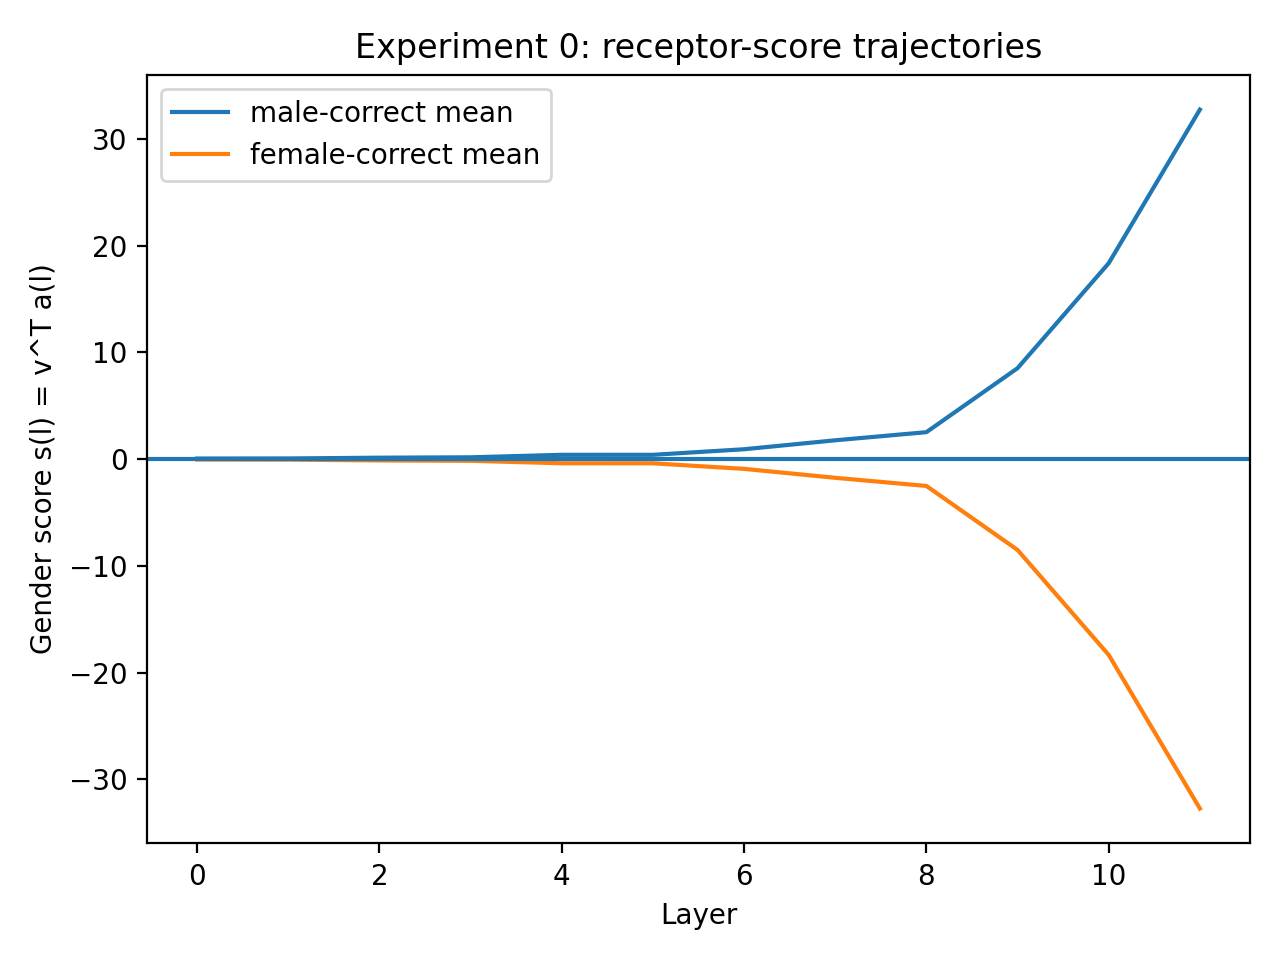
\includegraphics[width=\textwidth]{exp0_center_score_traj.png}
\caption{Receptor score trajectories (centered). Male and female means diverge sharply after layer 8.}
\label{fig:exp0_traj}
\end{subfigure}
\hfill
\begin{subfigure}[b]{0.48\textwidth}
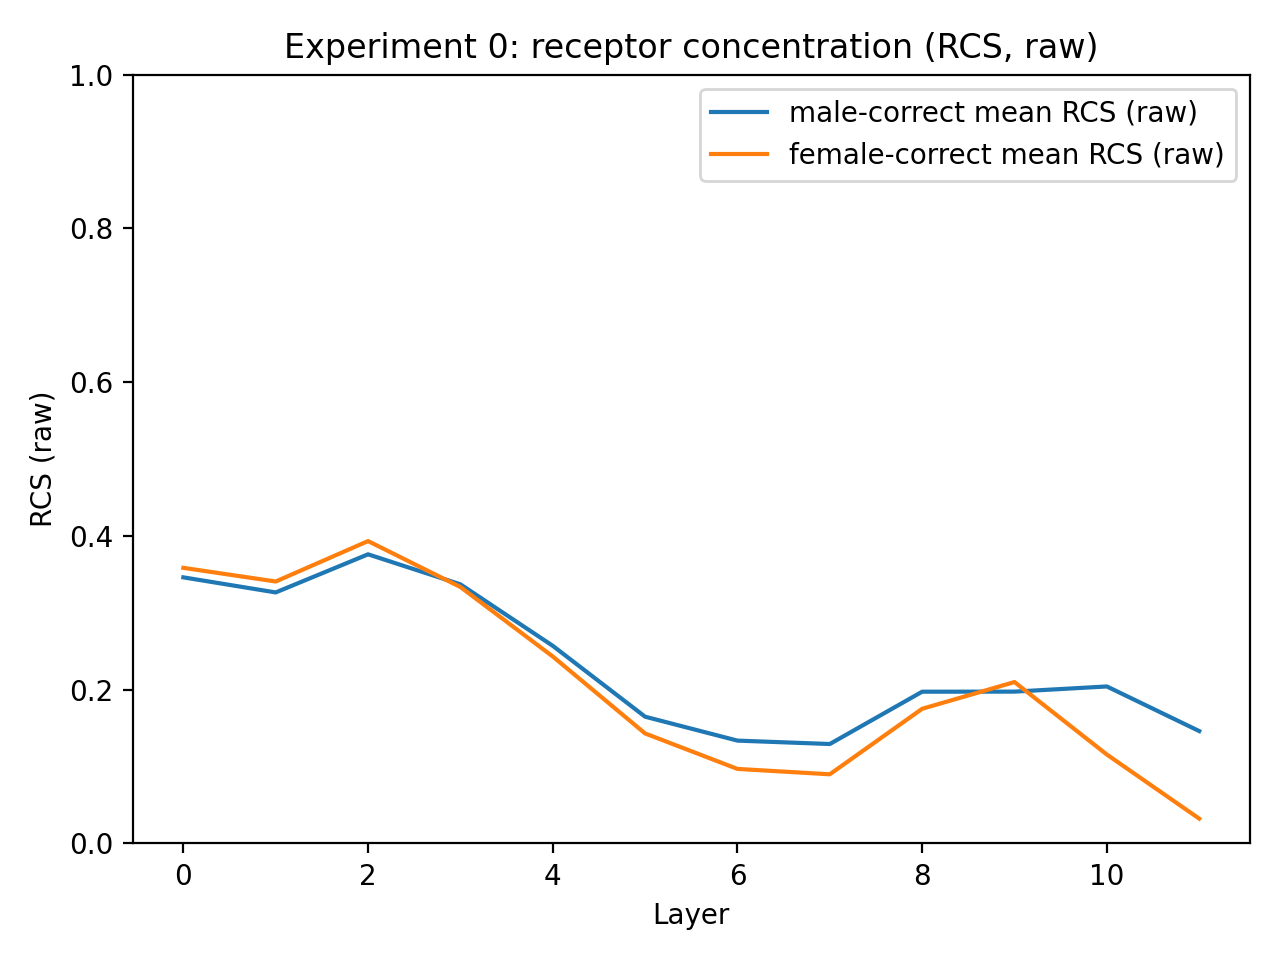
\includegraphics[width=\textwidth]{exp0_center_score_rcs_raw.png}
\caption{RCS by gender (raw). Early layers show higher concentration ($\sim 0.35$); late layers show more distributed contributions.}
\label{fig:exp0_rcs}
\end{subfigure}
\caption{Experiment 0: baseline diagnostics. Left: gender score trajectories separate after layer 8. Right: receptor concentration decreases across layers, meaning the circuit transitions from single-receptor dominance to distributed computation.}
\label{fig:exp0}
\end{figure}

The trajectory plot (Figure~\ref{fig:exp0_traj}) shows near-zero separation from layers 0--5, then a sharp divergence starting at layer 8--9. By layer 11, male-correct examples reach $s \approx +33$ and female-correct reach $s \approx -33$. The raw (uncentered) trajectories (Figure~\ref{fig:exp0_rcs}) show the same pattern with an overall negative offset.

The per-layer AUC (from the printed results) rises monotonically:

\begin{table}[H]
\centering
\small
\begin{tabular}{lcccccccccccc}
\toprule
Layer & 0 & 1 & 2 & 3 & 4 & 5 & 6 & 7 & 8 & 9 & 10 & 11 \\
\midrule
AUC & 0.58 & 0.61 & 0.65 & 0.66 & 0.67 & 0.68 & 0.78 & 0.79 & 0.82 & \textbf{0.95} & 0.96 & 0.96 \\
\bottomrule
\end{tabular}
\caption{Per-layer AUC of the combined receptor score $s(\ell)$ for gender classification.}
\label{tab:exp0_auc}
\end{table}

The jump from 0.82 (layer 8) to 0.95 (layer 9) coincides with R3's host head L9H7. This is the first indication that layer 9 is where the circuit ``turns on.''

Baseline model accuracy: 91.3\% (he-vs-she only), with 15.4\% of examples having a non-pronoun top-1 prediction.


%======================================================================
\section{Experiment 0c: Commitment Analysis}
\label{sec:exp0c}
%======================================================================

I wanted to know \emph{when} each receptor commits to its final sign. The commitment layer is the earliest layer $\ell$ where receptor $k$'s sign agrees with its final-layer sign for $\geq 85\%$ of examples, and this agreement is maintained at all subsequent layers.

Formally, for receptor $k$ at layer $\ell$:
\begin{equation}
\text{agree}_k(\ell) = \frac{1}{N}\sum_{i=1}^{N} \mathbf{1}\big[\text{sign}(g_k^{(\ell)}(i)) = \text{sign}(g_k^{(11)}(i))\big]
\end{equation}
The commitment layer is $L_k^* = \min\{\ell : \text{agree}_k(\ell') \geq 0.85 \;\forall\; \ell' \geq \ell\}$.

I also tracked three other diagnostics per layer:
\begin{itemize}[nosep]
\item \textbf{AUC}: ROC-AUC of $p_k \cdot g_k(\ell)$ for gender classification.
\item \textbf{Delta}: mean $|\Delta g_k| = |g_k(\ell+1) - g_k(\ell)|$, measuring where signal is written.
\item \textbf{Deliberation Index}: within-class variance of $g_k(\ell)$, normalized by layer $-1$.
\end{itemize}

\subsection{Results}

\begin{figure}[H]
\centering
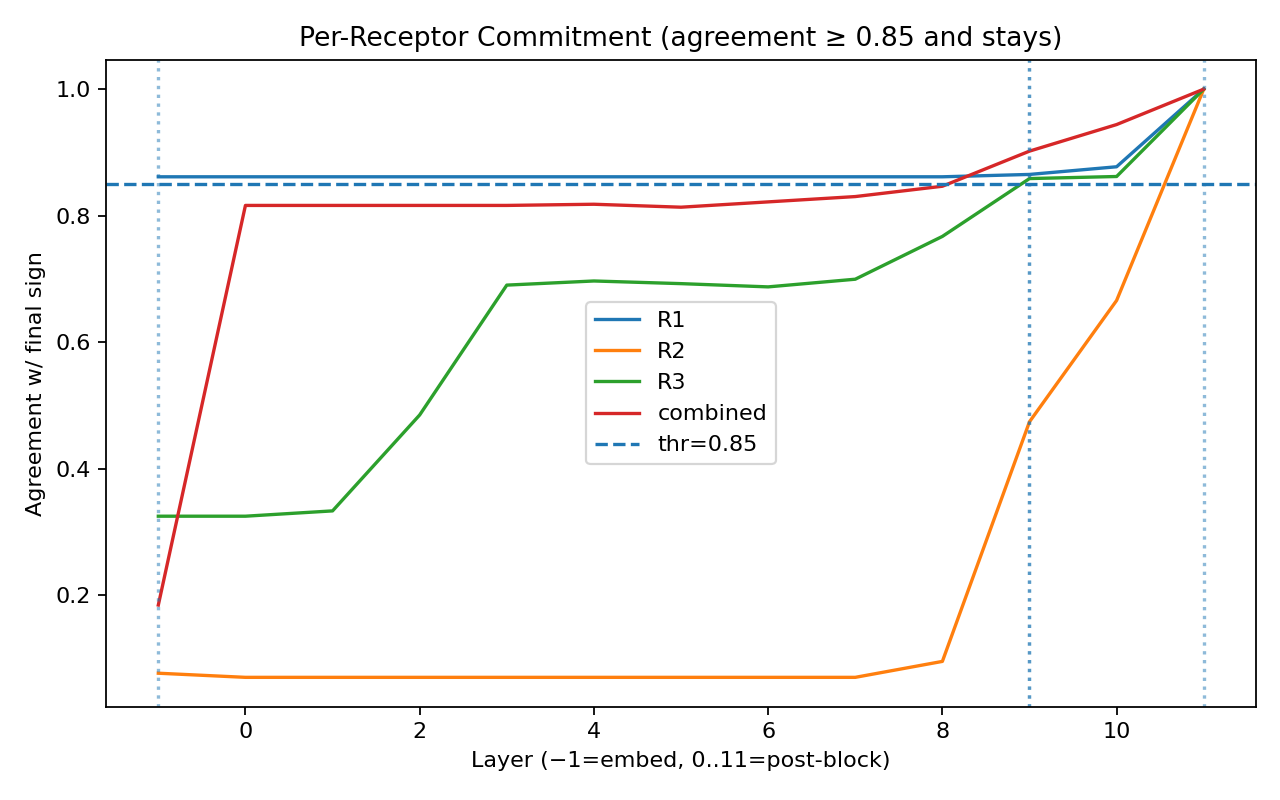
\includegraphics[width=0.7\textwidth]{commitment_plotpng.png}
\caption{Per-receptor commitment curves. R1 (blue) is committed from the embedding layer ($\ell = -1$). R3 (green) commits at layer 9. R2 (orange) commits only at layer 10--11. The dashed line marks the 0.85 threshold.}
\label{fig:commitment}
\end{figure}

The key finding: \textbf{R1 never has to ``commit'' because it is committed from the start.} Its sign agreement exceeds 0.85 from the embedding layer itself. This means R1 inherits its gender direction from the token embedding---it does not compute it. The name ``Brooks'' already projects positively onto R1's write direction before any attention head fires.

R3, by contrast, crosses 0.85 at layer 9, exactly where its host head L9H7 sits. R3 is a \emph{computed} signal. R2 commits even later (layer 10--11), consistent with its host head L11H8.

\begin{figure}[H]
\centering
\begin{subfigure}[b]{0.48\textwidth}
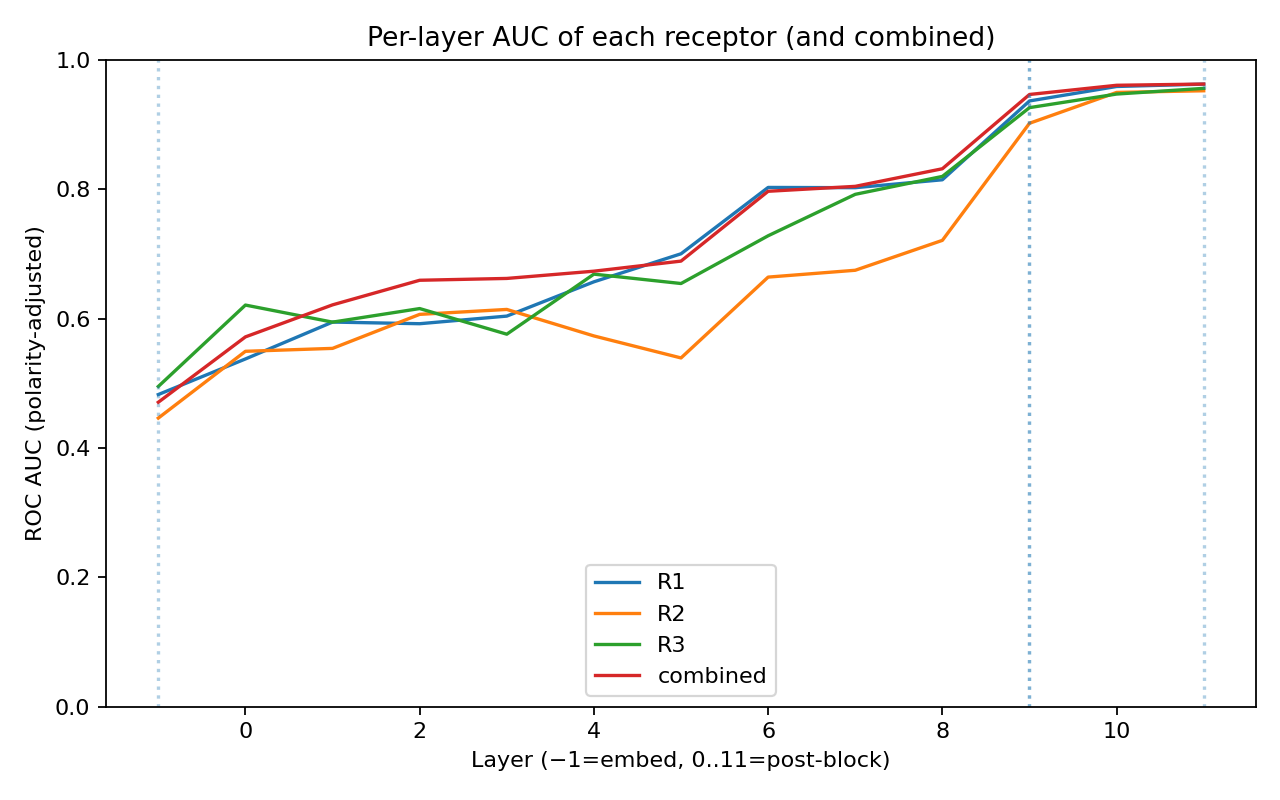
\includegraphics[width=\textwidth]{auc_plot.png}
\caption{Per-layer AUC. All receptors cross 0.90 at layer 9.}
\end{subfigure}
\hfill
\begin{subfigure}[b]{0.48\textwidth}
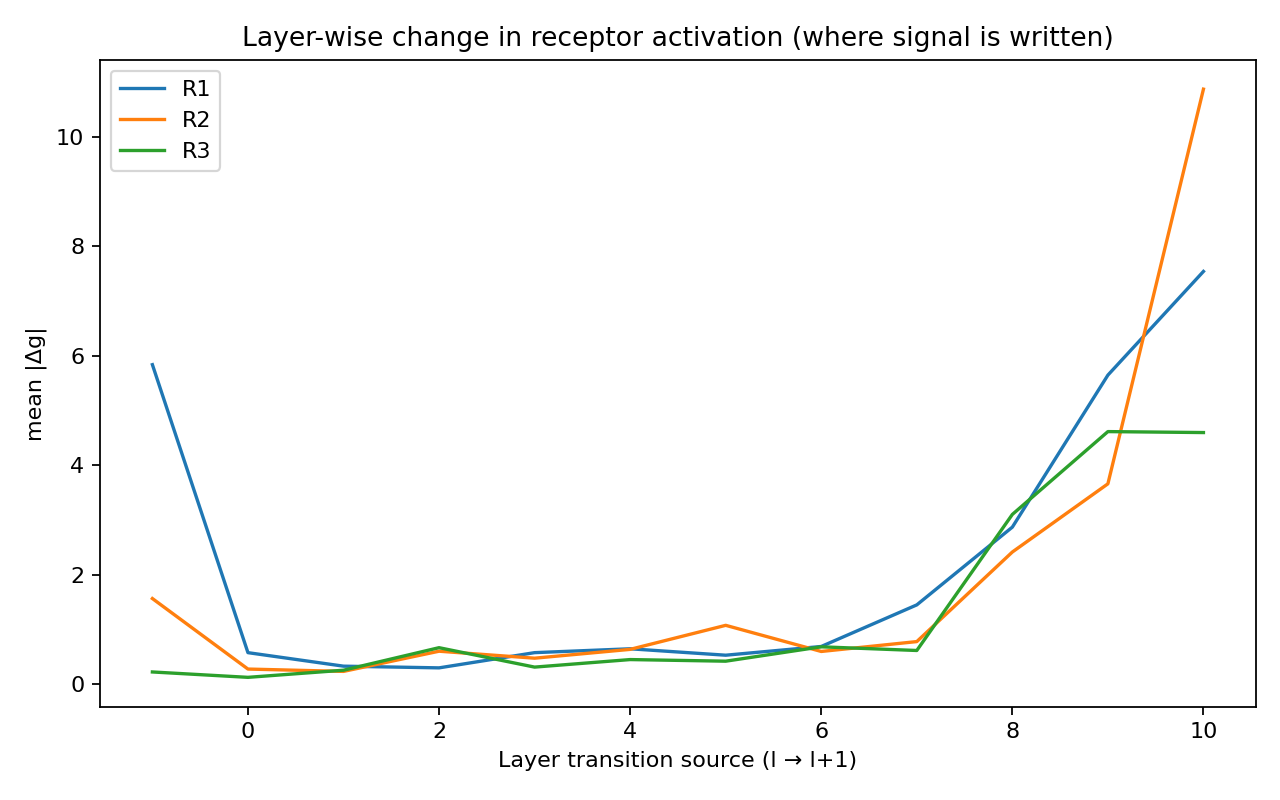
\includegraphics[width=\textwidth]{delta_by_layer.png}
\caption{Layer-wise $|\Delta g|$. R3 peaks at $9 \to 10$; R1 and R2 peak at $10 \to 11$.}
\end{subfigure}
\caption{AUC trajectories and delta peaks from Experiment 0c.}
\label{fig:exp0c_auc_delta}
\end{figure}

The delta peaks (Figure~\ref{fig:exp0c_auc_delta}b) serve as fingerprints: R3's signal is written at the $9 \to 10$ transition by its host head L9H7. R1's signal is amplified at $10 \to 11$ by L10H9. R2's signal appears at $10 \to 11$ as well, written by L11H8.

\begin{figure}[H]
\centering
\begin{subfigure}[b]{0.48\textwidth}
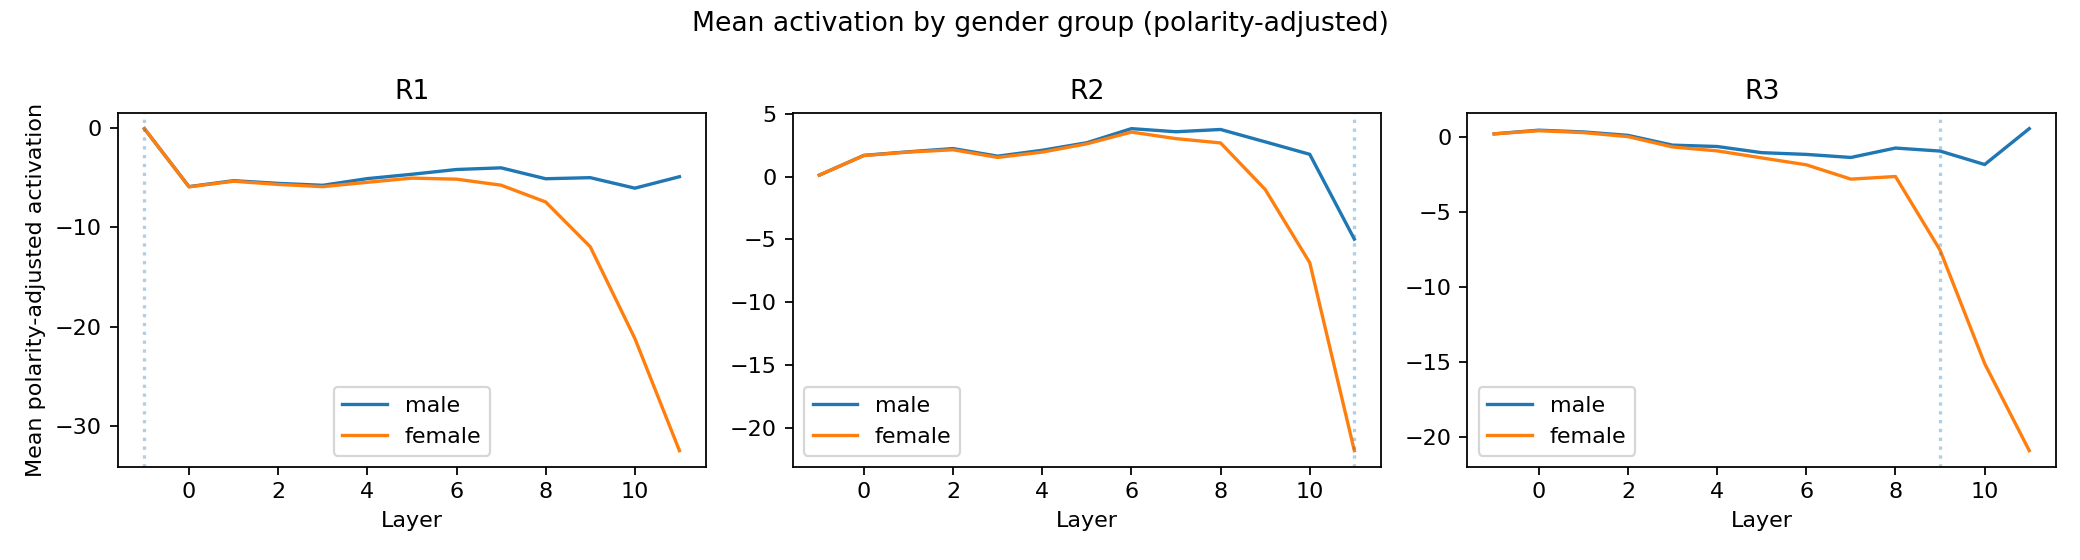
\includegraphics[width=\textwidth]{activation_by_gender.png}
\caption{Mean polarity-adjusted activation by gender group. R1 shows separation from the embedding. R3 separates at layer 9.}
\end{subfigure}
\hfill
\begin{subfigure}[b]{0.48\textwidth}
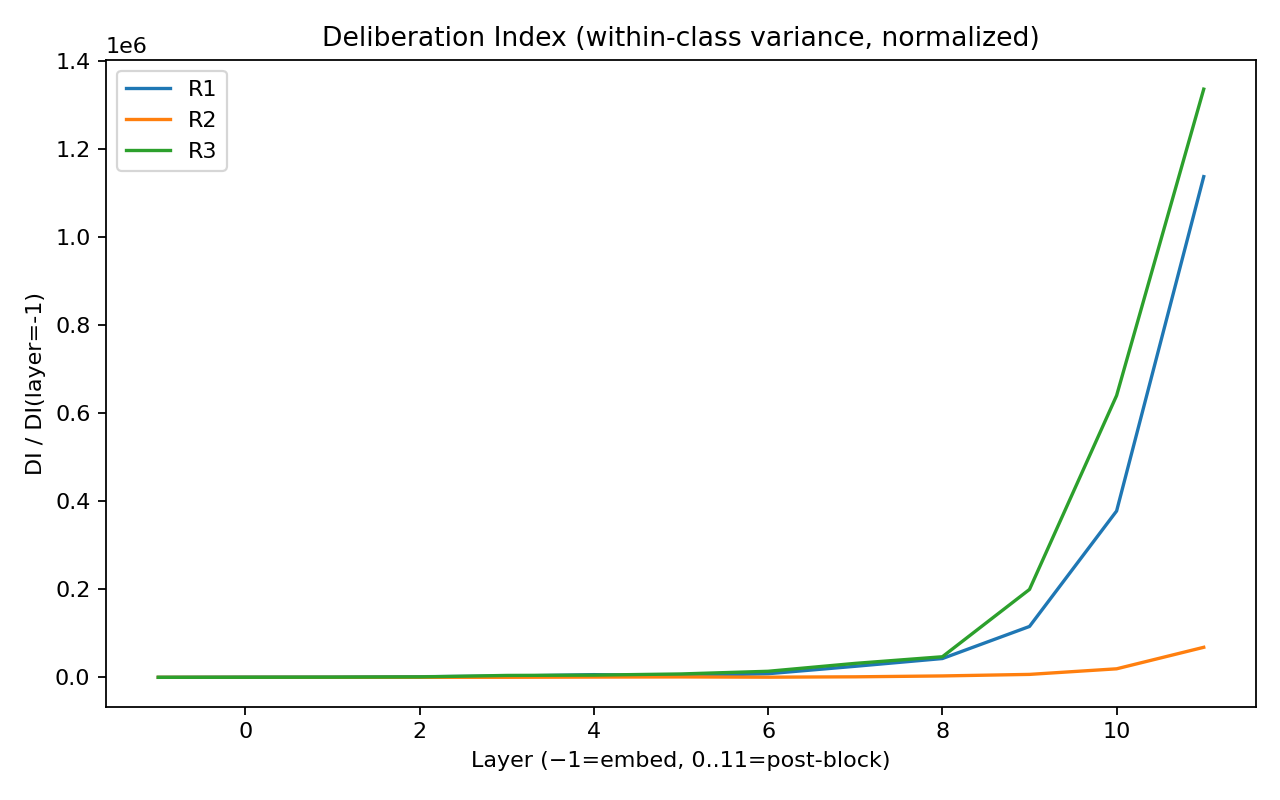
\includegraphics[width=\textwidth]{deliberation.png}
\caption{Deliberation index (within-class variance, normalized). Explodes at layers 9--11, reaching $10^6 \times$ the embedding variance.}
\end{subfigure}
\caption{Activation by gender and deliberation from Experiment 0c.}
\label{fig:exp0c_gender_delib}
\end{figure}

The deliberation explosion (Figure~\ref{fig:exp0c_gender_delib}b) is striking. Within-class variance grows by a factor of $\sim 10^6$ from the embedding to the final layer. This means late layers do not just separate genders---they amplify individual differences within each gender class. This amplification creates both the strong correct predictions (large margins) and the failures on ambiguous names (names that happen to get amplified in the wrong direction).

\paragraph{Interpretation.} The circuit has an \emph{inherited-vs-computed asymmetry}. R1's signal is free: the embedding already contains gender information along R1's direction. R3's signal is computed: L9H7 must actively write it. This asymmetry has consequences for robustness---R1 is reliable but coarse, R3 is powerful but fragile.

\begin{figure}[H]
\centering
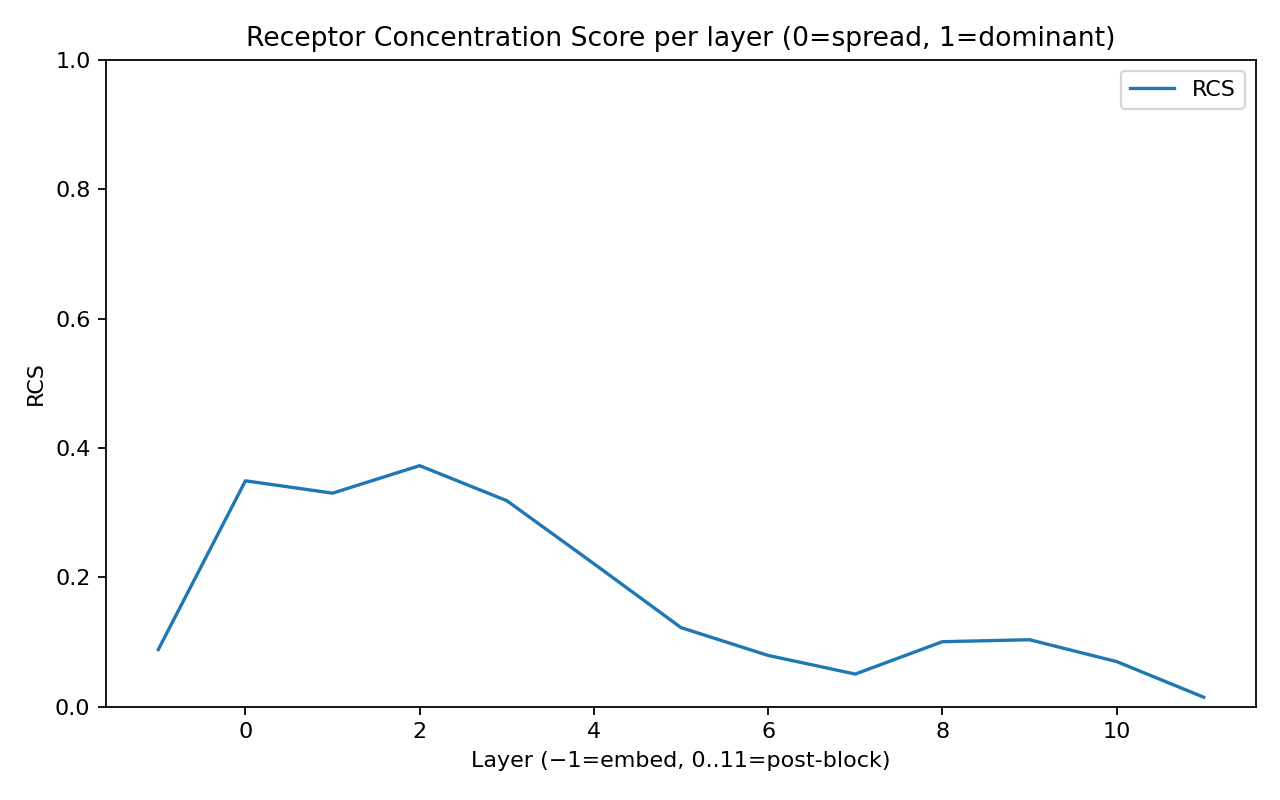
\includegraphics[width=0.6\textwidth]{rcs.png}
\caption{Receptor Concentration Score per layer (from Experiment 0c). RCS peaks around layers 0--2 ($\sim$0.37) and drops to near zero at layer 11. The circuit moves from single-receptor dominance to distributed computation.}
\label{fig:rcs_0c}
\end{figure}


%======================================================================
\section{Experiment 2: Cross-Talk Under Scaling}
\label{sec:exp2}
%======================================================================

R1 and R3 have cosine similarity $-0.775$. When I scale R3's activation, R1's activation changes. But is this change purely geometric (because $v_1$ and $v_3$ are not orthogonal) or does it reflect genuine computational coupling (R3's perturbation propagates through intermediate layers and changes R1's output)?

I disentangle these two effects. When I scale receptor $k$ by factor $s$, receptor $j$'s activation changes by $\Delta g_j$. The geometric prediction is:
\begin{equation}
\Delta g_j^{\text{geo}} = (s-1) \cdot \sigma_k \cdot \bar{a}_k \cdot \cos(v_k, v_j)
\end{equation}
This is what would happen if the perturbation passed through without any nonlinear processing. The \emph{computational fraction} is:
\begin{equation}
\text{CompFrac}(k \to j) = 1 - \frac{|\Delta g_j^{\text{geo}}|}{|\Delta g_j^{\text{actual}}|}
\end{equation}
If CompFrac $= 0$, all cross-talk is geometric. If CompFrac $> 0$, there is computational coupling beyond geometry.

I ran this at scales $s \in \{0.1, 0.5, 1.0, 2.0, 5.0, 10.0, 20.0\}$ and measured cross-talk at each.

\subsection{Results}

\begin{figure}[H]
\centering
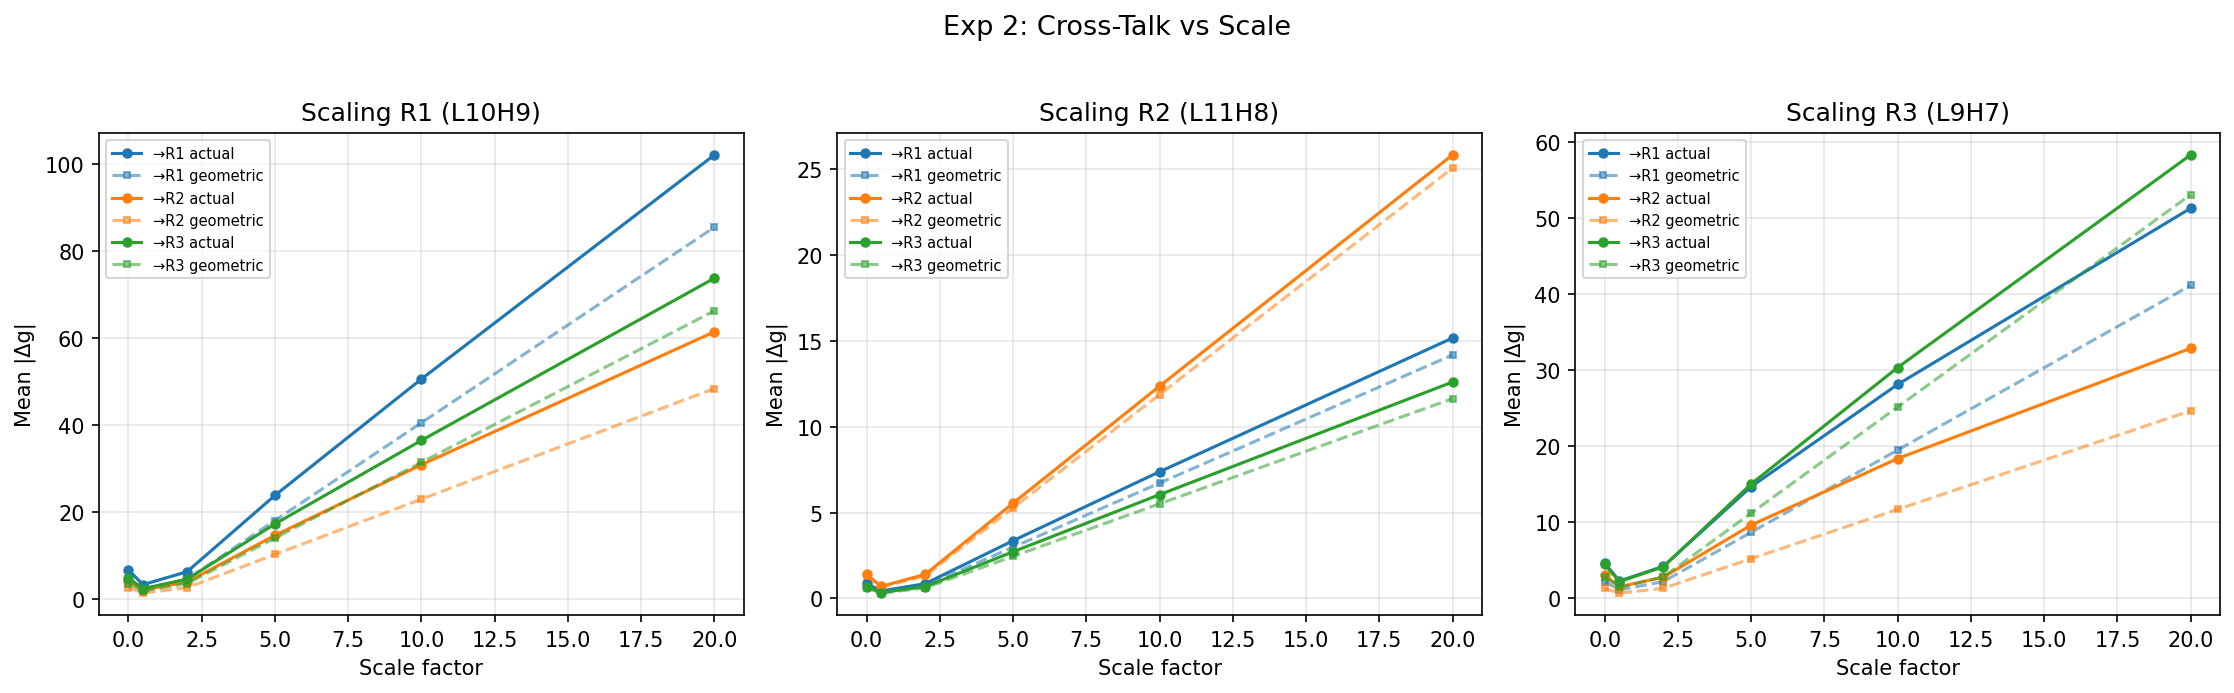
\includegraphics[width=\textwidth]{exp2_crosstalk_vs_scale.png}
\caption{Cross-talk vs.\ scale for all source--target pairs. Solid lines: actual $|\Delta g|$. Dashed lines: geometric prediction. The gap between solid and dashed is the computational component.}
\label{fig:exp2_scale}
\end{figure}

\begin{figure}[H]
\centering
\begin{subfigure}[b]{0.45\textwidth}
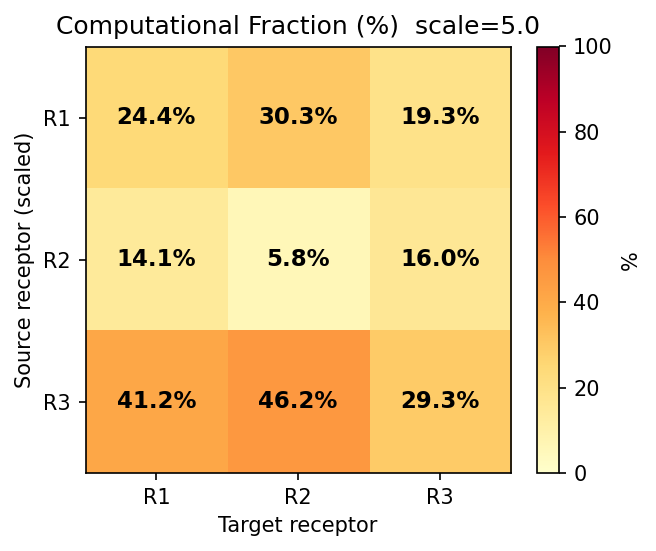
\includegraphics[width=\textwidth]{exp2_comp_fraction.png}
\caption{Computational fraction matrix at scale 5.0.}
\label{fig:exp2_compfrac}
\end{subfigure}
\hfill
\begin{subfigure}[b]{0.48\textwidth}
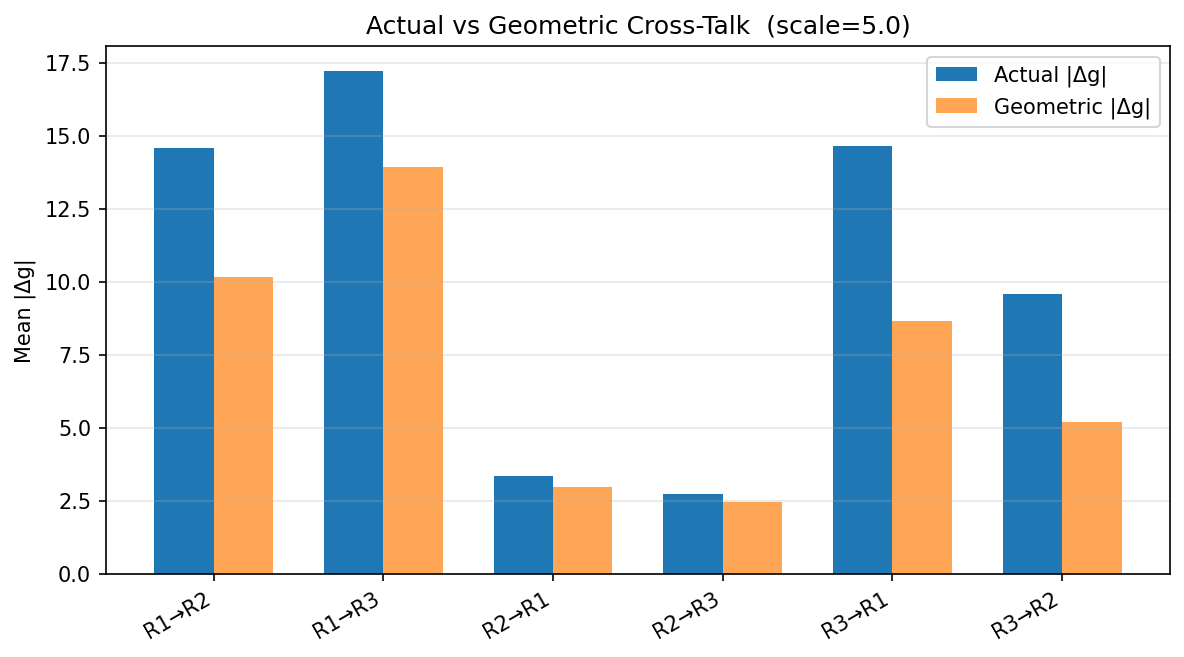
\includegraphics[width=\textwidth]{exp2_actual_vs_geometric.png}
\caption{Actual vs.\ geometric $|\Delta g|$ at scale 5.0.}
\label{fig:exp2_actual_geo}
\end{subfigure}
\caption{Experiment 2: cross-talk decomposition.}
\label{fig:exp2}
\end{figure}

The computational fraction matrix (Figure~\ref{fig:exp2_compfrac}) reveals clear structure:

\begin{table}[H]
\centering
\begin{tabular}{lccc}
\toprule
Source $\to$ Target & R1 & R2 & R3 \\
\midrule
R1 $\to$ & 24.4\% & 30.3\% & 19.3\% \\
R2 $\to$ & 14.1\% & 5.8\%  & 16.0\% \\
R3 $\to$ & \textbf{41.2\%} & \textbf{46.2\%} & 29.3\% \\
\bottomrule
\end{tabular}
\caption{Computational fraction at scale 5.0. R3 $\to$ R1 coupling is 41.2\%---nearly half the effect is computational.}
\label{tab:compfrac}
\end{table}

Three findings stand out:

\textbf{R2's self-CompFrac is 5.8\%.} R2's host head L11H8 is in the last layer; after it writes, only $\text{ln\_final}$ remains. The perturbation passes through almost unchanged. This is a clean control: the methodology works.

\textbf{R3 $\to$ R1 CompFrac is 41.2\%.} When R3 (L9H7) is scaled, 41\% of the resulting change in R1 cannot be explained by geometry. The perturbation at layer 9 passes through layers 10 and 11, and L10H9 (R1's host head) reads the modified residual and recomputes. This is genuine computational coupling.

\textbf{The asymmetry is confirmed.} R3 $\to$ R1 CompFrac (41.2\%) exceeds R1 $\to$ R3 CompFrac (19.3\%). This is expected: R3's host head fires before R1's, so R3's perturbation flows \emph{through} R1's head, but not vice versa. I predicted this asymmetry before running the experiment; the data confirms it.

Linearity check: R$^2$ of mean $|\Delta g|$ vs.\ $|s-1|$ exceeds 0.99 for all pairs, confirming the perturbation regime is linear.


%======================================================================
\section{Experiment 4: Shapley Ablation and Independence}
\label{sec:exp4}
%======================================================================

I wanted to quantify each receptor's individual contribution. Shapley values provide a principled decomposition. For each subset $S \subseteq \{R1, R2, R3\}$, I project out the directions \emph{not} in $S$ from the final residual stream, then recompute logits via $\text{ln\_final}$ and $W_U$.

The Shapley value for receptor $k$ on metric $v$ (accuracy or mean margin) is:
\begin{equation}
\phi_k = \frac{1}{K!} \sum_{\pi} \big[v(S_\pi^k \cup \{k\}) - v(S_\pi^k)\big]
\end{equation}
where the sum is over all orderings $\pi$ of the $K=3$ receptors, and $S_\pi^k$ is the set of receptors preceding $k$ in ordering $\pi$.

With $K=3$, there are $2^3 = 8$ coalitions. I evaluated all eight.

\subsection{Results}

\begin{table}[H]
\centering
\begin{tabular}{lcccc}
\toprule
Coalition & Acc (he-vs-she) & Top-1 Acc & Mean margin & RCS \\
\midrule
NONE (all ablated)  & 0.816 & 0.722 & +0.975 & 0.031 \\
R1 only             & 0.879 & 0.764 & +1.985 & 0.023 \\
R2 only             & 0.809 & 0.716 & +1.065 & 0.031 \\
R3 only             & 0.849 & 0.748 & +1.537 & 0.021 \\
R1+R2               & 0.876 & 0.765 & +2.103 & 0.022 \\
R1+R3               & 0.890 & 0.769 & +2.450 & 0.015 \\
R2+R3               & 0.853 & 0.752 & +1.643 & 0.020 \\
R1+R2+R3 (baseline) & 0.889 & 0.771 & +2.579 & 0.015 \\
\bottomrule
\end{tabular}
\caption{Coalition accuracies and margins from Experiment 4.}
\label{tab:exp4_coalitions}
\end{table}

\begin{figure}[H]
\centering
\begin{subfigure}[b]{0.48\textwidth}
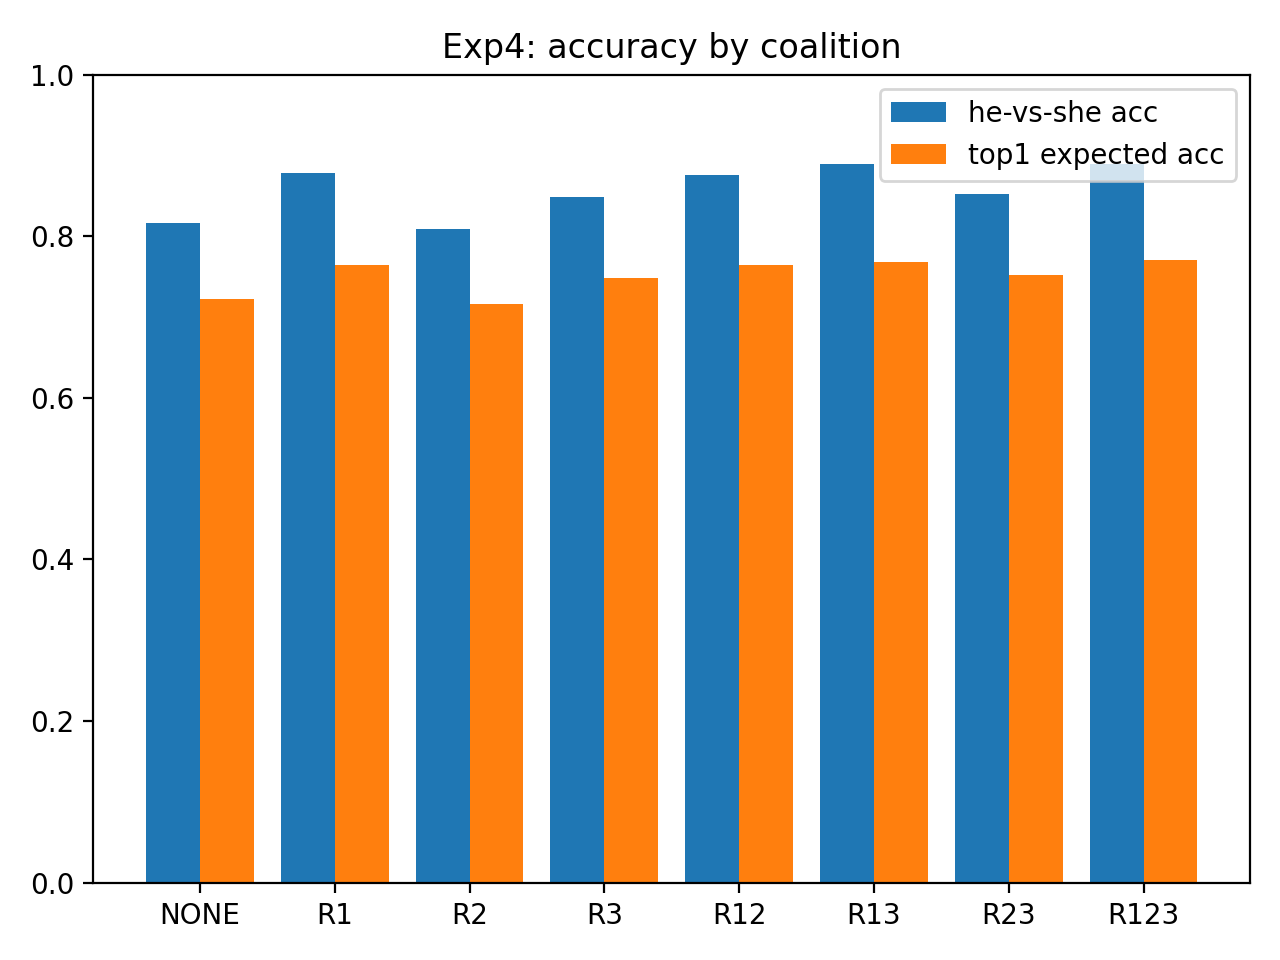
\includegraphics[width=\textwidth]{exp4_acc.png}
\caption{Accuracy by coalition.}
\end{subfigure}
\hfill
\begin{subfigure}[b]{0.48\textwidth}
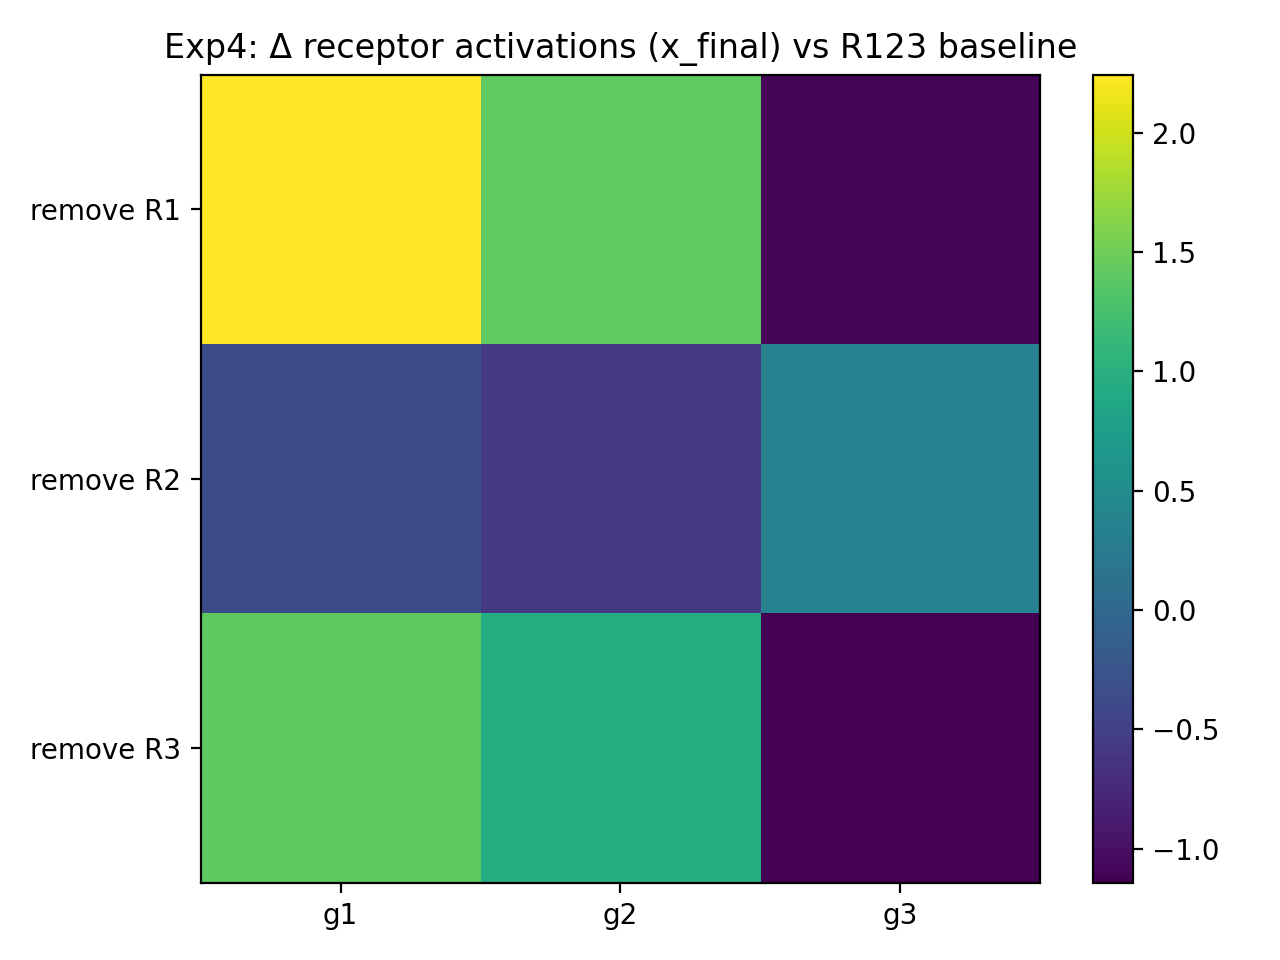
\includegraphics[width=\textwidth]{exp4_delta_acts.png}
\caption{$\Delta$ activations when removing each receptor.}
\end{subfigure}
\caption{Experiment 4: Shapley ablation results.}
\label{fig:exp4}
\end{figure}

The Shapley values for accuracy are: $\phi_\text{acc}(R1) = +0.051$, $\phi_\text{acc}(R2) = -0.003$, $\phi_\text{acc}(R3) = +0.024$. For mean margin: $\phi_\text{margin}(R1) = +0.974$, $\phi_\text{margin}(R2) = +0.110$, $\phi_\text{margin}(R3) = +0.520$.

\textbf{R2 contributes essentially nothing.} Its accuracy Shapley value is $-0.003$ (removing it actually helps slightly), and its margin Shapley is only 0.110 out of 1.604 total. This was the first quantitative evidence that R2 is a ghost---a direction that appears gender-aligned in logit space but contributes negligibly to the task.

\textbf{R1 dominates margin.} R1's margin Shapley (0.974) is nearly twice R3's (0.520). R1 is the primary driver of confident predictions.

The interaction indices confirm anti-cooperative behavior between R1 and R3: $I_{13}(\text{acc}) = -0.011$, $I_{13}(\text{margin}) = -0.048$. Having both provides slightly less than the sum of their individual contributions, consistent with their anti-correlated directions partially canceling.


%======================================================================
\section{Phase Diagram and Error Autopsy}
\label{sec:phase}
%======================================================================

I next built a decision landscape. For each example $i$, define the \emph{R1 margin} as $m_1(i) = y_i \cdot p_1 \cdot g_1^{(11)}(i)$ and the \emph{R3 margin} as $m_3(i) = y_i \cdot p_3 \cdot g_3^{(11)}(i)$, where $y_i \in \{+1, -1\}$ is the label. Positive margin means the receptor votes correctly.

Plotting $m_1$ vs.\ $m_3$ for all examples gives a phase diagram. Errors can be classified by which receptor failed:

\begin{itemize}[nosep]
\item \textbf{Type B (inhibition failure):} R1 correct ($m_1 > 0$), R3 wrong ($m_3 < 0$). R3 failed to suppress.
\item \textbf{Type C (both fail):} $m_1 < 0$ and $m_3 < 0$.
\item \textbf{Type D (margin failure):} Both correct ($m_1 > 0$, $m_3 > 0$), but combined margin too small; other logit components overwhelm.
\end{itemize}

(Type A, promotion-only failure with $m_1 < 0$ and $m_3 > 0$, did not occur.)

\subsection{Results}

\begin{figure}[H]
\centering
\begin{subfigure}[b]{0.48\textwidth}
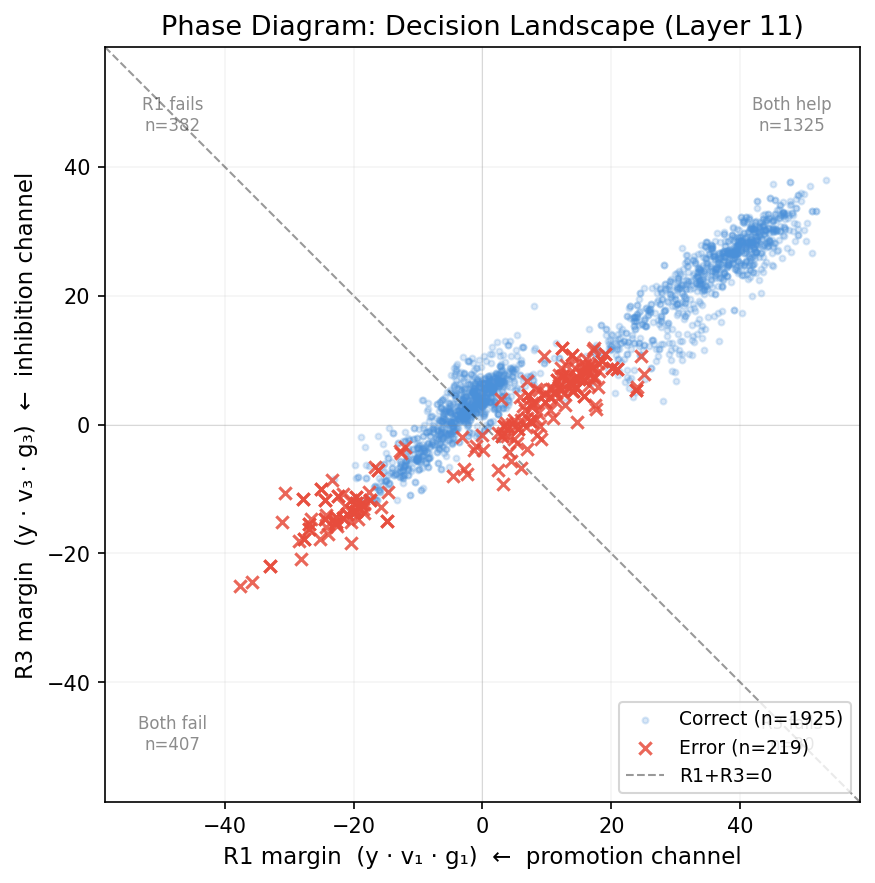
\includegraphics[width=\textwidth]{phase_diagram.png}
\caption{Phase diagram at final layer. Blue dots: correct. Red crosses: errors. Errors cluster near the origin (low margins).}
\label{fig:phase_diagram}
\end{subfigure}
\hfill
\begin{subfigure}[b]{0.48\textwidth}
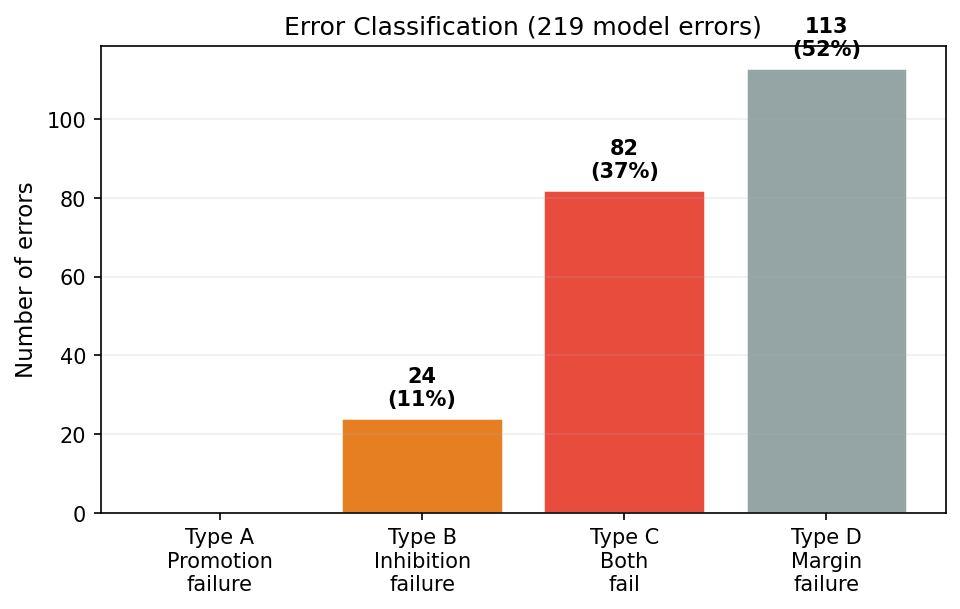
\includegraphics[width=\textwidth]{error_types.png}
\caption{Error classification. 219 total errors: Type B = 24 (11\%), Type C = 82 (37\%), Type D = 113 (52\%).}
\label{fig:error_types}
\end{subfigure}
\caption{Phase diagram and error autopsy.}
\label{fig:phase}
\end{figure}

\begin{figure}[H]
\centering
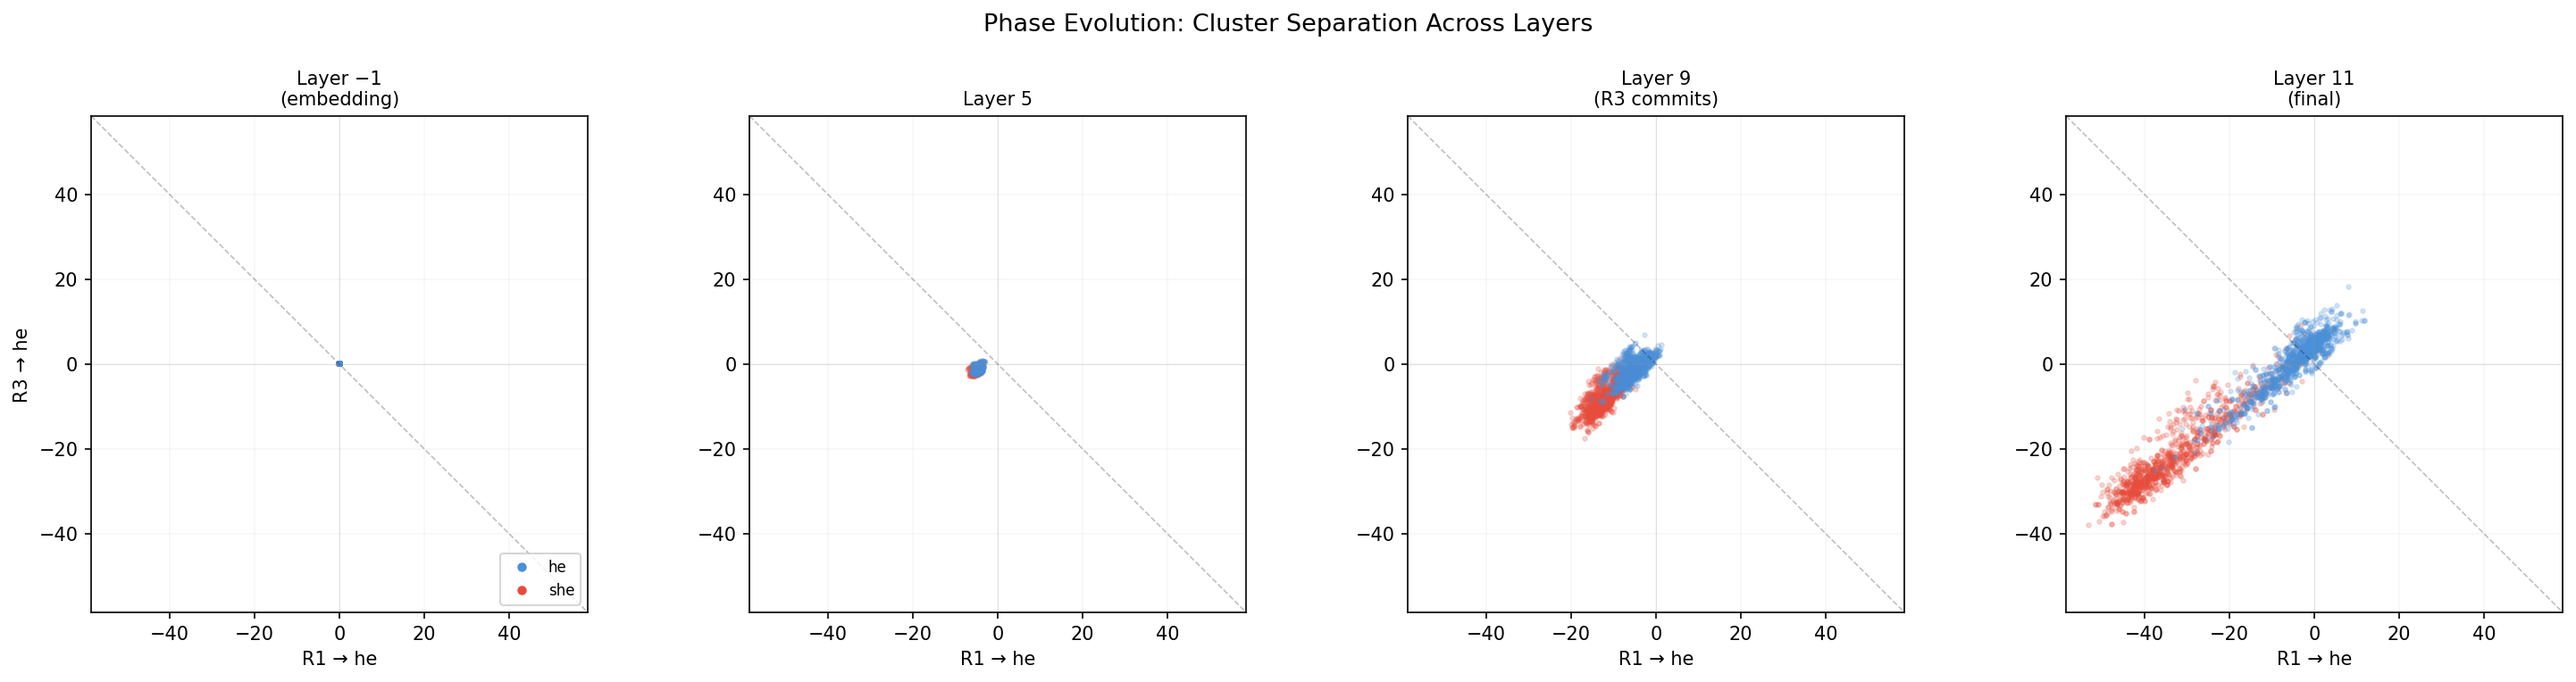
\includegraphics[width=\textwidth]{phase_evolution.png}
\caption{Phase evolution across layers. At layer $-1$ (embedding), all points are clustered near the origin. By layer 9, gender clusters emerge. By layer 11, full separation.}
\label{fig:phase_evolution}
\end{figure}

The error breakdown surprised me. I expected Type B (inhibition failure) to dominate, because R3 is the computed, fragile channel. Instead, \textbf{Type D (margin failure) is the majority at 52\%}. In these 113 cases, both R1 and R3 vote correctly, but their combined margin is small enough that other logit components push the model's prediction the wrong way.

Type C (both fail, 37\%) corresponds to genuinely ambiguous names. In these cases, the name's embedding already points the wrong direction on both R1 and R3.

\begin{figure}[H]
\centering
\begin{subfigure}[b]{0.48\textwidth}
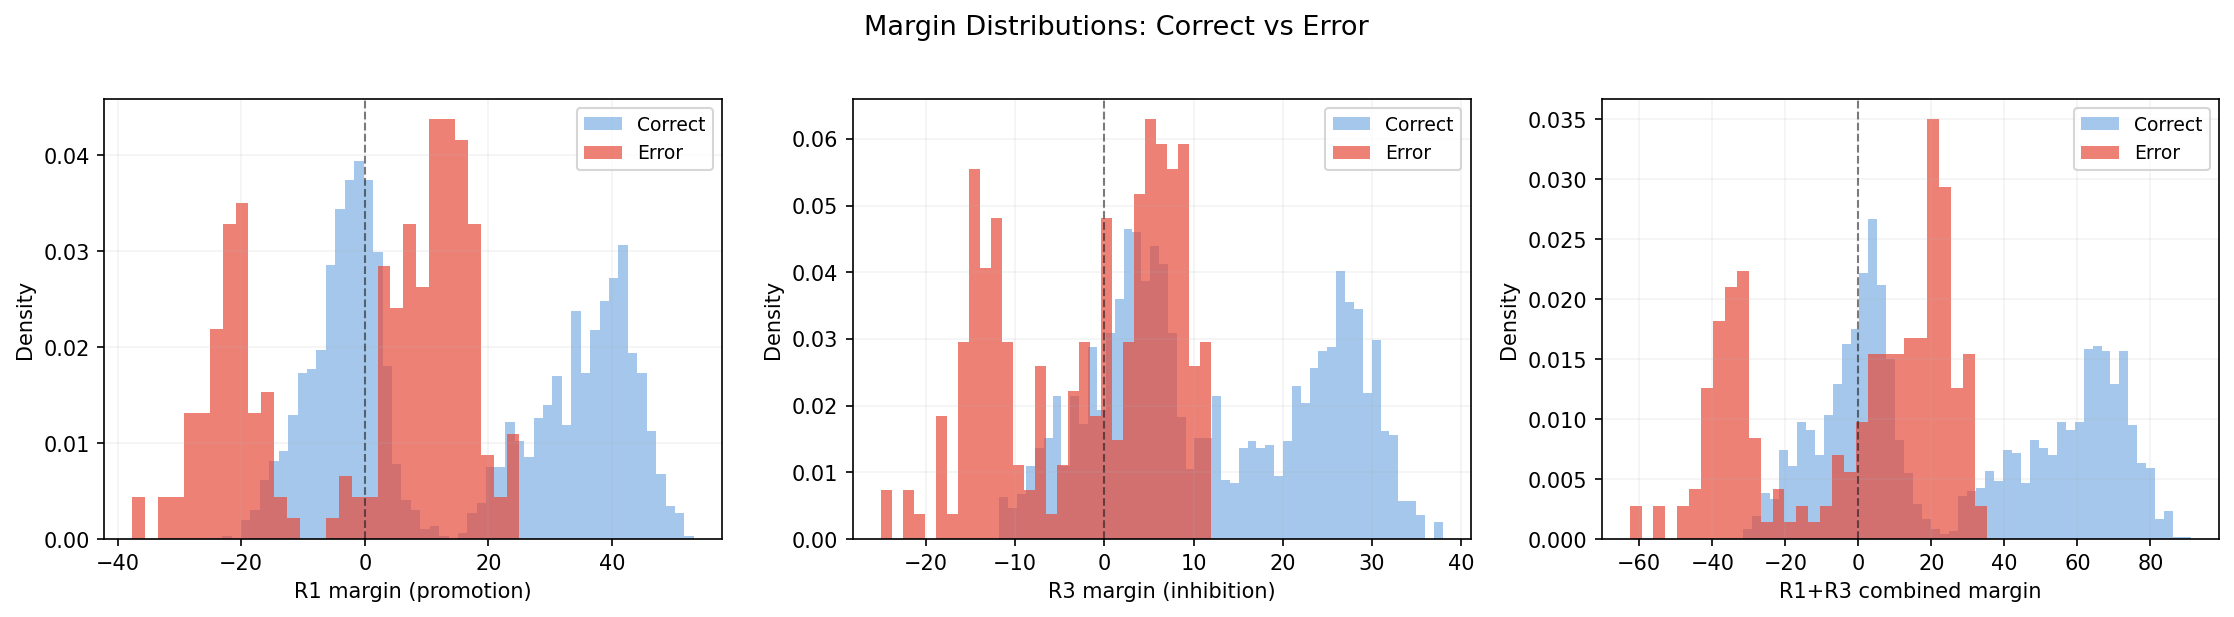
\includegraphics[width=\textwidth]{margin_histograms.png}
\caption{Margin distributions for correct vs.\ error examples.}
\end{subfigure}
\hfill
\begin{subfigure}[b]{0.48\textwidth}
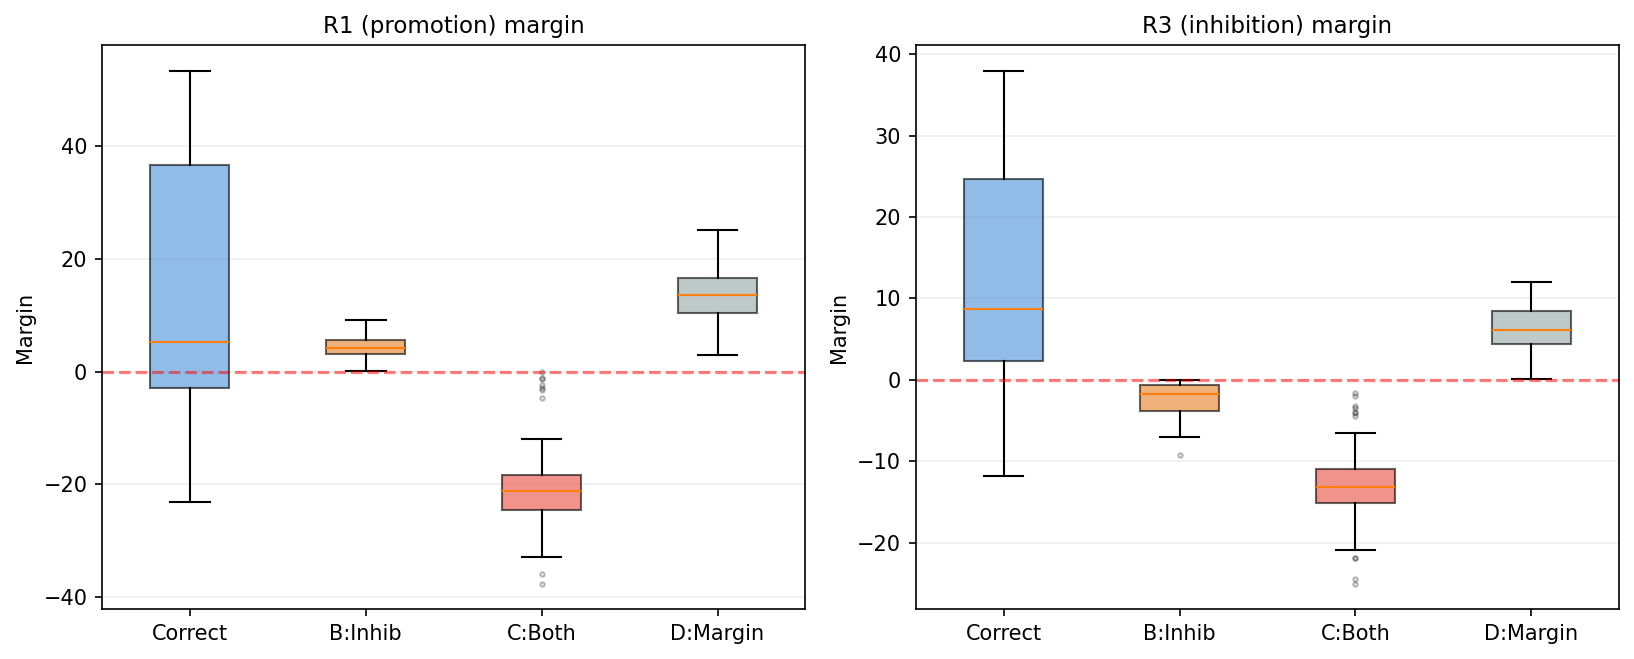
\includegraphics[width=\textwidth]{margin_by_error_type.png}
\caption{Per-receptor margins by error type.}
\end{subfigure}
\caption{Margin analysis. Errors are concentrated near zero margin. Type C errors show strongly negative margins on both receptors. Type D errors show positive but small margins.}
\label{fig:margins}
\end{figure}

The margin distributions (Figure~\ref{fig:margins}a) confirm that error examples are clustered near zero combined margin. The circuit coverage (Figure~\ref{fig:circuit_coverage}) shows that roughly 35\% of model errors have negative R1+R3 margin across all layers, dropping from 65\% at the embedding.

\begin{figure}[H]
\centering
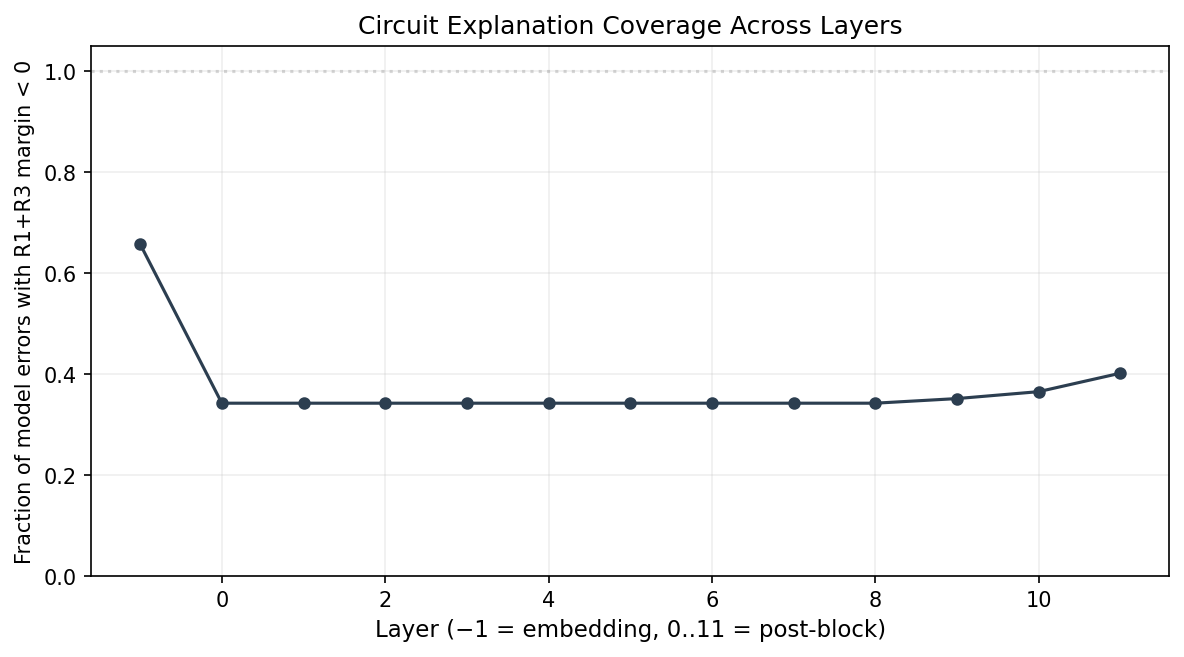
\includegraphics[width=0.6\textwidth]{circuit_coverage.png}
\caption{Circuit explanation coverage across layers. Fraction of model errors where R1+R3 margin is negative. Drops from 0.65 at the embedding to $\sim$0.35 at later layers.}
\label{fig:circuit_coverage}
\end{figure}


%======================================================================
\section{Type D Gap Analysis}
\label{sec:typed}
%======================================================================

The 113 Type D errors raise a natural question: if both receptors vote correctly, \emph{what} is overriding them? I decompose the model's logit difference into a receptor component and a residual:
\begin{equation}
\underbrace{\text{logit}(\text{he}) - \text{logit}(\text{she})}_{\text{model decision}} = \underbrace{(v_1^\top x) \cdot w_1 + (v_3^\top x) \cdot w_3}_{\text{receptor subspace}} + \underbrace{\text{remainder}}_{\text{other components}}
\end{equation}
where $w_k$ are the projections of the unembedding difference vector onto the receptor directions.

More precisely, I project the final residual stream $x^{(11)}$ onto the 3-receptor subspace $\text{span}(v_1, v_2, v_3)$ and its orthogonal complement. The receptor score is $\hat{s} = p_1 g_1 + p_3 g_3$ (ignoring R2 since $\phi(R2) \approx 0$).

\subsection{Results}

\begin{figure}[H]
\centering
\begin{subfigure}[b]{0.48\textwidth}
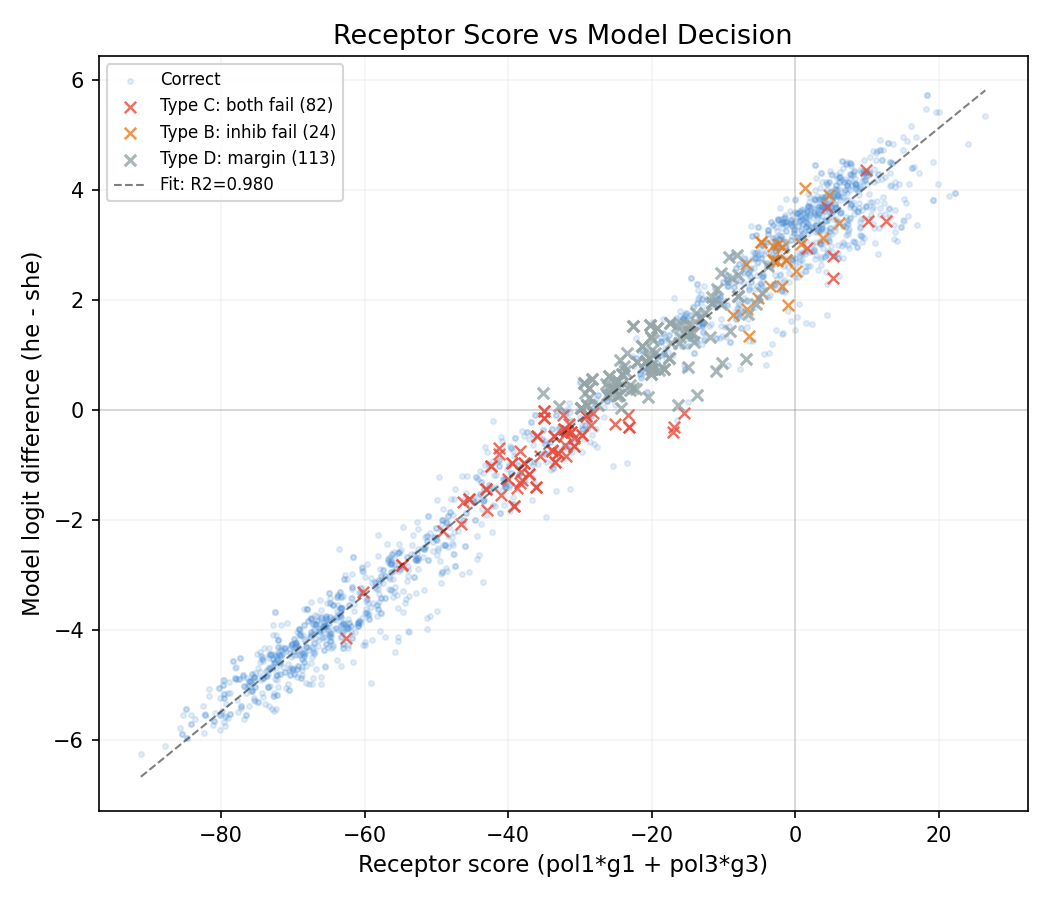
\includegraphics[width=\textwidth]{typed_scatter.png}
\caption{Receptor score vs.\ model logit difference. $R^2 = 0.980$. Error types are color-coded.}
\label{fig:typed_scatter}
\end{subfigure}
\hfill
\begin{subfigure}[b]{0.48\textwidth}
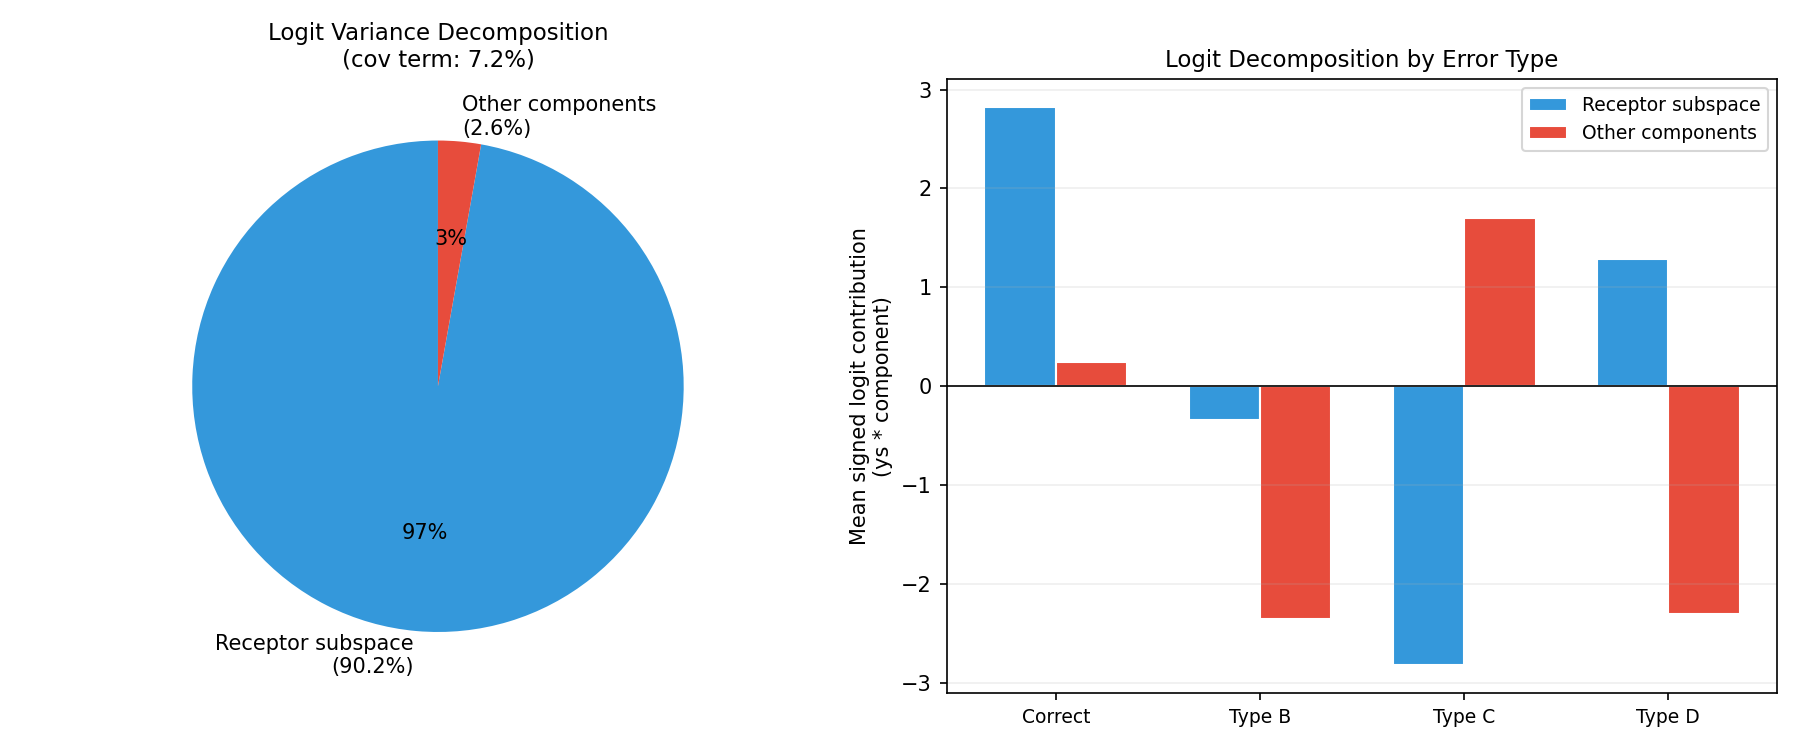
\includegraphics[width=\textwidth]{typed_variance_pie.png}
\caption{Variance decomposition. Receptor subspace explains 90.2\% of logit variance.}
\label{fig:typed_pie}
\end{subfigure}
\caption{Type D gap analysis.}
\label{fig:typed}
\end{figure}

\textbf{The two-receptor model explains 98.0\% of the variance in the model's logit difference} ($R^2 = 0.980$). The receptor subspace accounts for 90.2\% of total logit variance; the orthogonal complement accounts for 2.6\%; the covariance term is 7.2\%.

\begin{figure}[H]
\centering
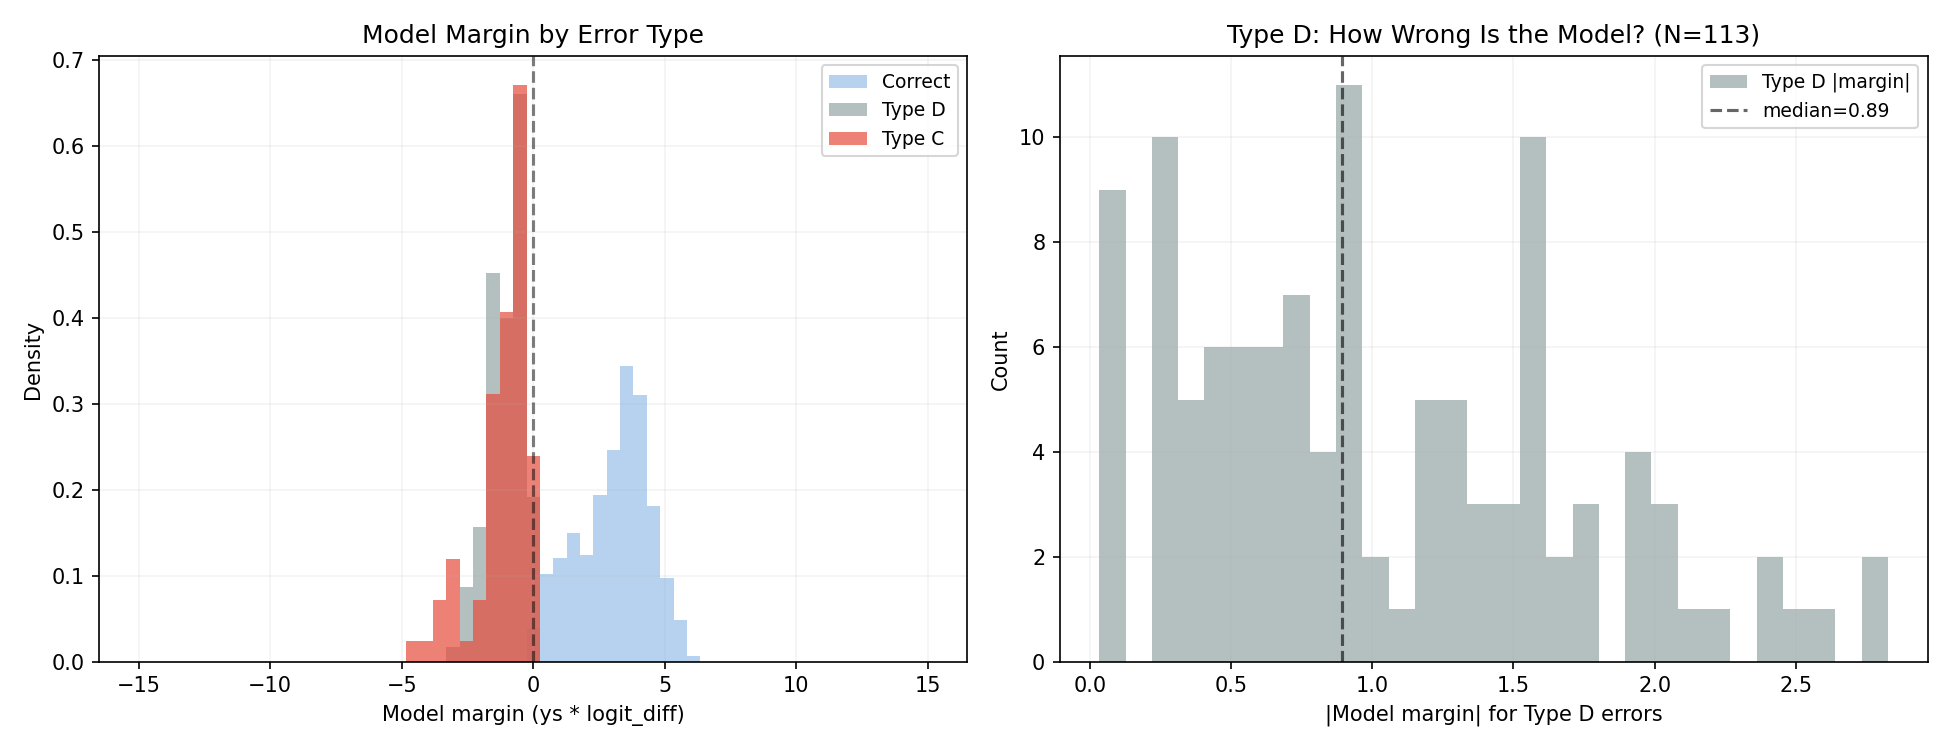
\includegraphics[width=0.85\textwidth]{typed_margin_dist.png}
\caption{Left: model margin by error type. Type D errors are clustered near zero. Right: absolute model margin for Type D errors. Median is 0.89---these are razor-thin losses.}
\label{fig:typed_margin_dist}
\end{figure}

For the 113 Type D errors specifically, the median absolute model margin is 0.89 logit units. The model is barely wrong. These are cases where the receptor circuit gives the right answer, but the 2.6\% residual (other logit components) tips the balance. The logit decomposition by error type (Figure~\ref{fig:typed_pie} right panel) shows that for correct examples, the receptor subspace contributes positively and the residual is small. For Type C errors, the receptor subspace itself is negative. For Type D errors, the receptor subspace is positive but small, and the residual pushes negative.


%======================================================================
\section{Experiment 5: Cross-Structure Generalization}
\label{sec:exp5}
%======================================================================

All experiments so far used one sentence structure: ``So [Name] is a very [adj] person, isn't \_\_''. I needed to test whether the receptor directions generalize across syntactic contexts. I constructed five sentence structures:

\begin{itemize}[nosep]
\item \textbf{A: Tag question} (baseline): ``So [Name] is a very [adj] person, isn't \_\_''
\item \textbf{B: Because}: ``Because [Name] is [adj], \_\_''
\item \textbf{C: Temporal}: ``After [Name] finished the project, \_\_''
\item \textbf{D: Prep-of}: ``A friend of [Name] said that \_\_''
\item \textbf{E: Cross-sentence}: ``[Name] is [adj]. \_\_''
\end{itemize}

For each structure, I generated $\sim$1200 examples using the same name pool, ran a forward pass, and measured receptor AUC at the decision position.

\subsection{Results}

\begin{figure}[H]
\centering
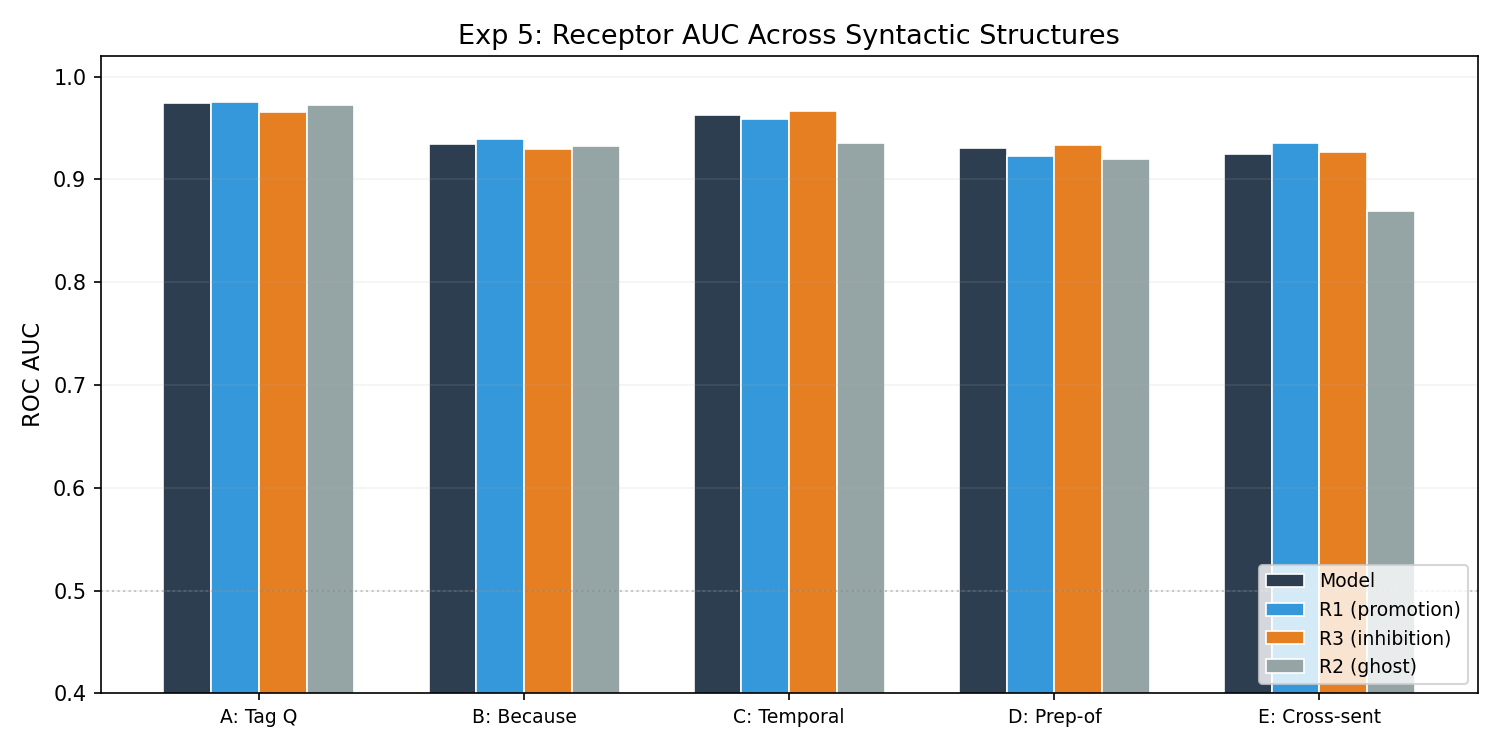
\includegraphics[width=0.8\textwidth]{exp5_auc_bars.png}
\caption{Receptor AUC across five syntactic structures. All remain above 0.92 for R1 and R3. R2 (ghost) drops to 0.87 on cross-sentence.}
\label{fig:exp5_auc}
\end{figure}

\textbf{All structures maintain AUC $\geq 0.92$ for R1, R3, and the model.} The generalization gap (Figure~\ref{fig:exp5_gen_drop}) shows drops of at most 5 percentage points from the baseline structure. The largest drop is R1 on structure D (Prep-of), which falls by $\sim$0.05.

\begin{figure}[H]
\centering
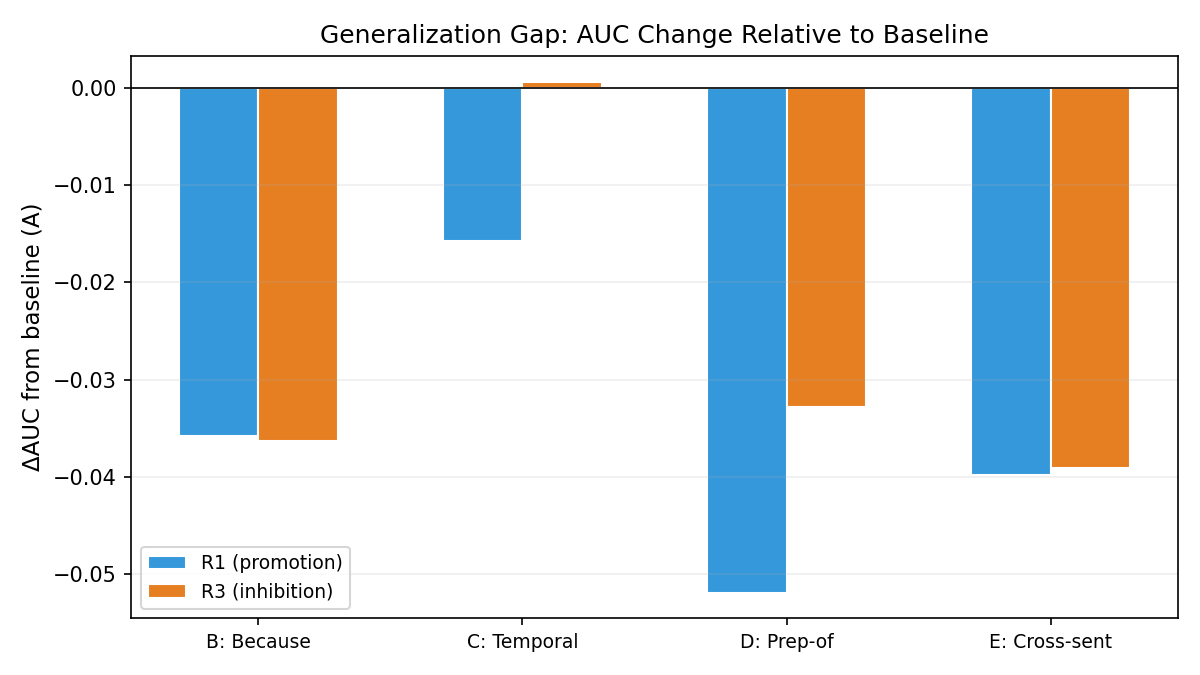
\includegraphics[width=0.7\textwidth]{exp5_gen_drop.png}
\caption{AUC drop relative to baseline (structure A). Maximum drop is $\sim$0.05 (R1 on Prep-of). R3 is most stable across structures.}
\label{fig:exp5_gen}
\end{figure}

The receptor directions generalize robustly. Even on cross-sentence structure (E), where the period token might reset attention patterns, AUC remains above 0.92 for R1 and R3.


%======================================================================
\section{Experiment 5b: Ambiguous Names}
\label{sec:exp5b}
%======================================================================

I extracted names from the dataset that appear in both male and female contexts, giving them a \emph{he-fraction} $\in (0,1)$. Names with he-fraction near 0.5 are ambiguous (e.g., Angel, Tyler, Christian). I measured receptor activations and model predictions for 128 ambiguous examples and compared them to 571 unambiguous examples.

\subsection{Results}

\begin{figure}[H]
\centering
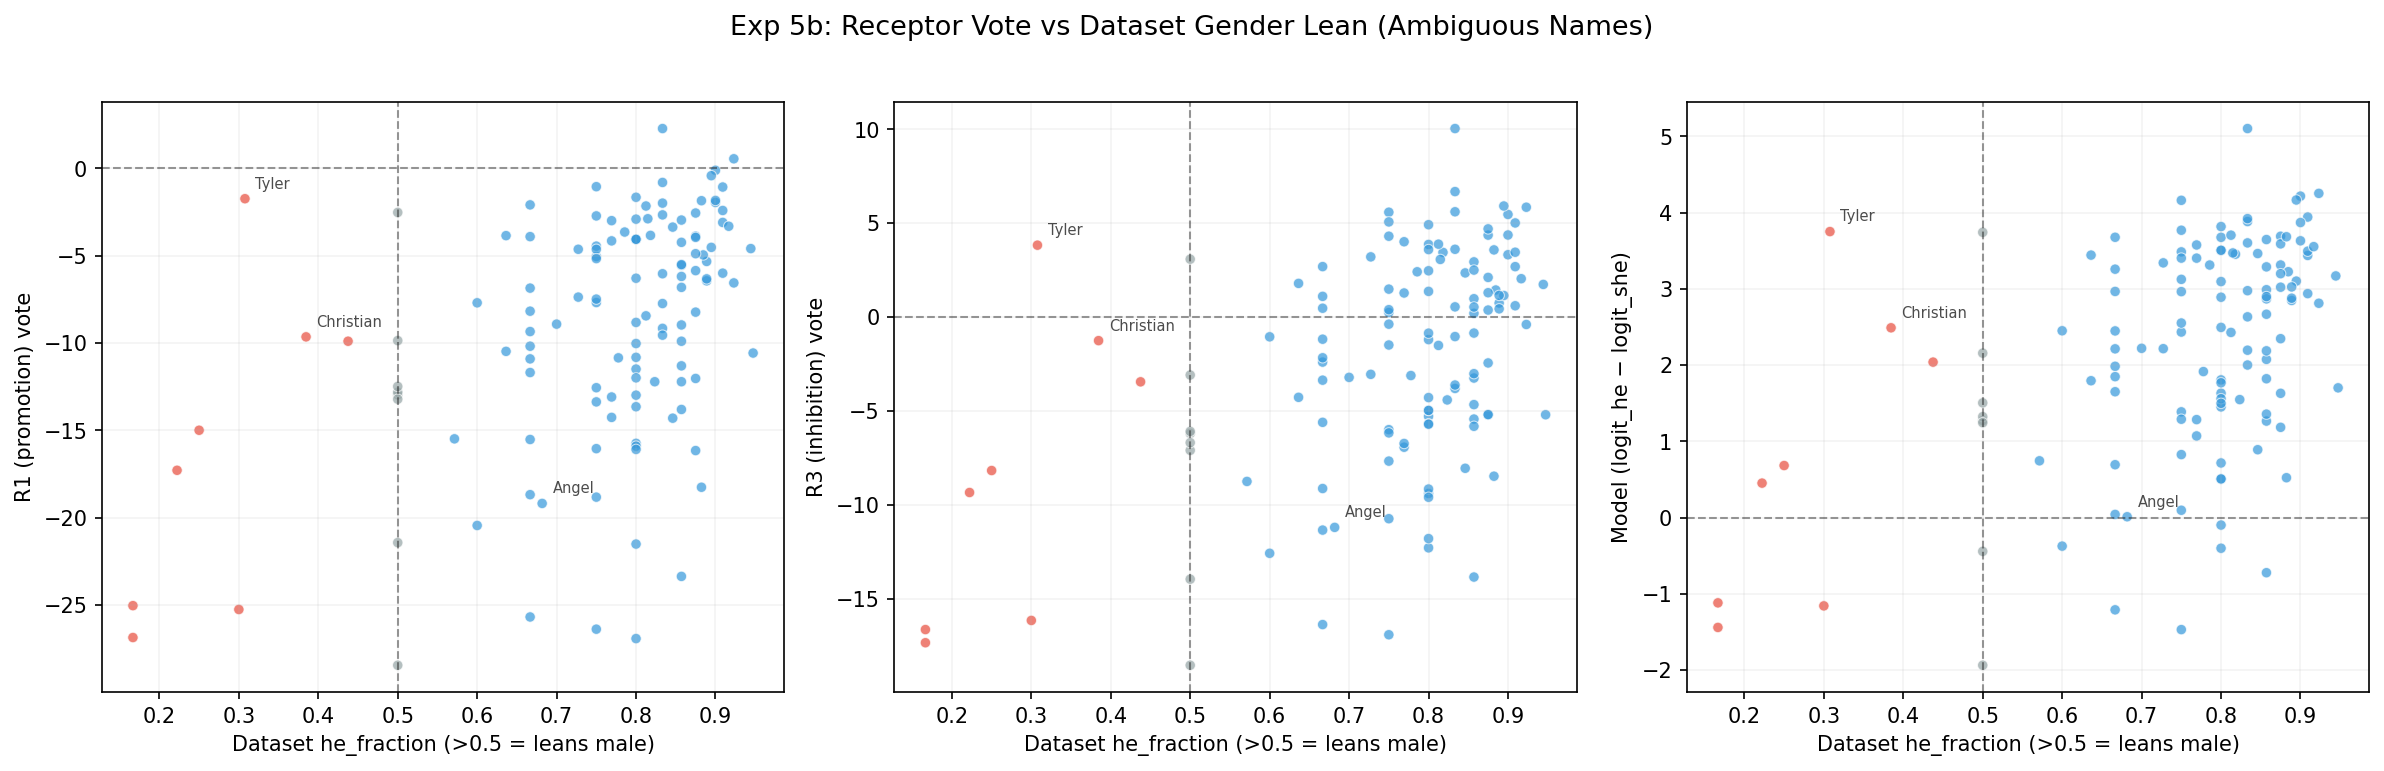
\includegraphics[width=\textwidth]{exp5b_ambig_scatter.png}
\caption{Receptor vote vs.\ dataset gender lean for ambiguous names. Left: R1 (promotion). Middle: R3 (inhibition). Right: model logit difference. Ambiguous names (gray, near $x=0.5$) cluster near the decision boundary. Tyler, Christian, and Angel are highlighted as particularly ambiguous.}
\label{fig:exp5b}
\end{figure}

AUC drops from $\sim$0.97 (unambiguous) to $\sim$0.75 (ambiguous) for all receptors and the model alike. The drop is uniform across R1, R3, R2, and the model. This means the performance loss is not a failure of any specific receptor---it is a property of the input. Ambiguous names project weakly onto both R1 and R3, producing small margins that are easily overwhelmed.

The scatter plot (Figure~\ref{fig:exp5b}b) shows that Tyler, Christian, and Angel are among the most ambiguous: their receptor activations are near the decision boundary regardless of the intended gender context. The model ``knows'' it does not know, in the sense that its confidence is low for these inputs.


%======================================================================
\section{Causal Fidelity Ratio: Ghost Detection}
\label{sec:cfr}
%======================================================================

The mask training identified 207 (layer, head, sv\_index) triples with nonzero mask weights. But Experiment~4 showed that R2 contributes nothing despite appearing gender-aligned. How many of the 207 are similarly hollow?

I define the \emph{Causal Fidelity Ratio} (CFR) to test each direction:
\begin{equation}
\text{CFR}_k = \frac{\text{AccDrop}(k)}{\text{AUC}_k - 0.5}
\end{equation}
where $\text{AccDrop}(k)$ is the accuracy drop when receptor $k$'s direction is projected out of the final residual stream, and $\text{AUC}_k$ measures how well the direction separates he-contexts from she-contexts. A direction with high AUC but zero AccDrop is a ghost: it ``looks'' gendered but removing it does not hurt. CFR captures this: ghosts have CFR $\approx 0$; real receptors have CFR $\gg 0$.

I tested all 207 directions on the 612-example test set, with a batch size of 8 and one forward pass per direction.

\subsection{Results}

\begin{figure}[H]
\centering
\begin{subfigure}[b]{0.48\textwidth}
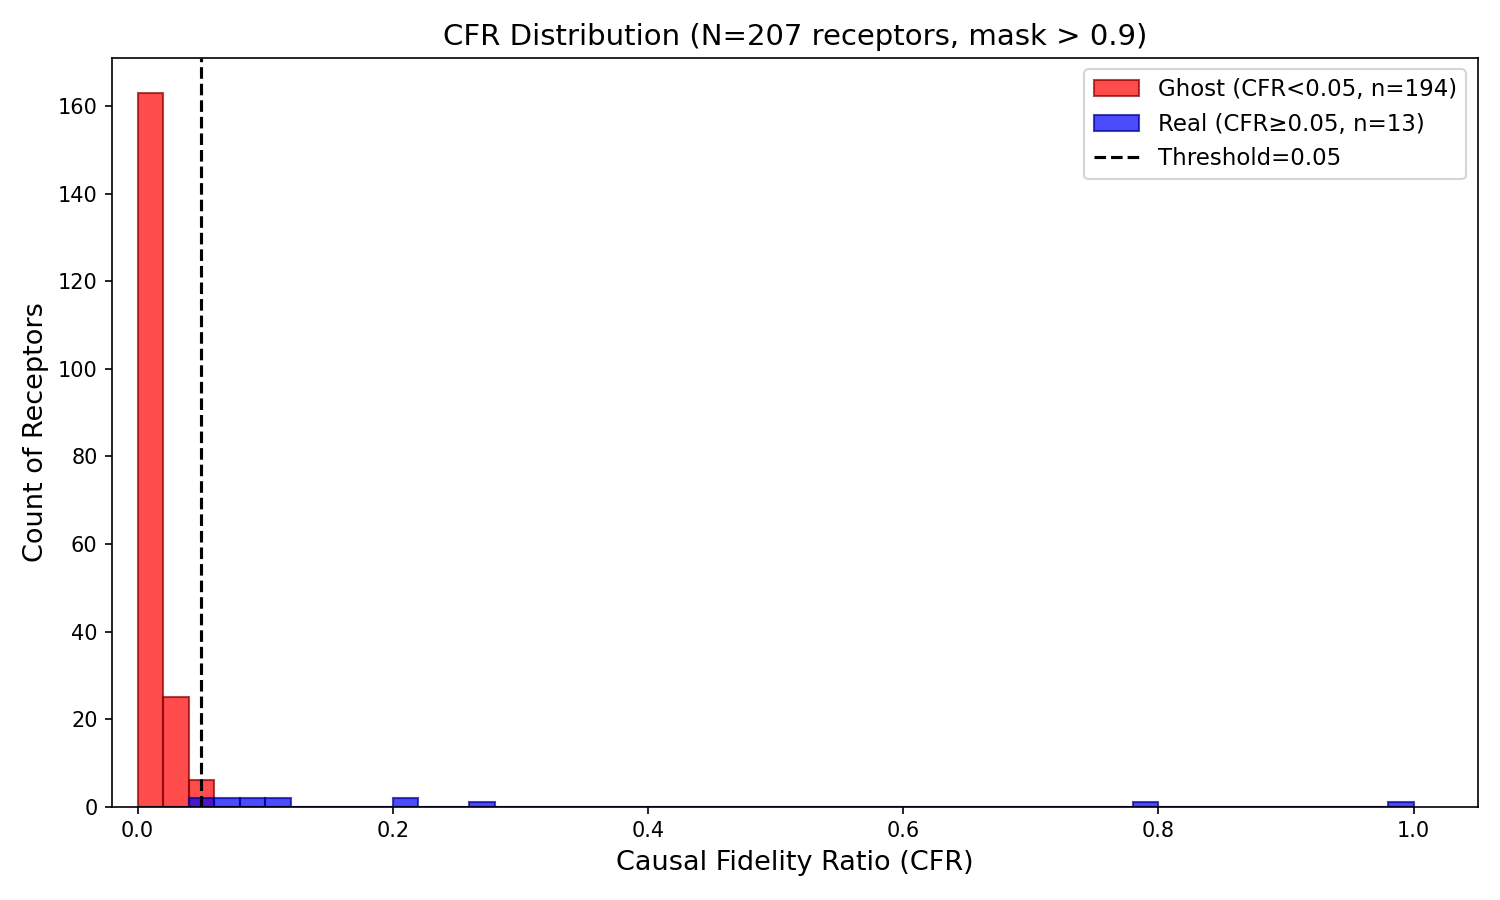
\includegraphics[width=\textwidth]{plot1_cfr_histogram.png}
\caption{CFR histogram. 194 of 207 directions have CFR $< 0.1$.}
\end{subfigure}
\hfill
\begin{subfigure}[b]{0.48\textwidth}
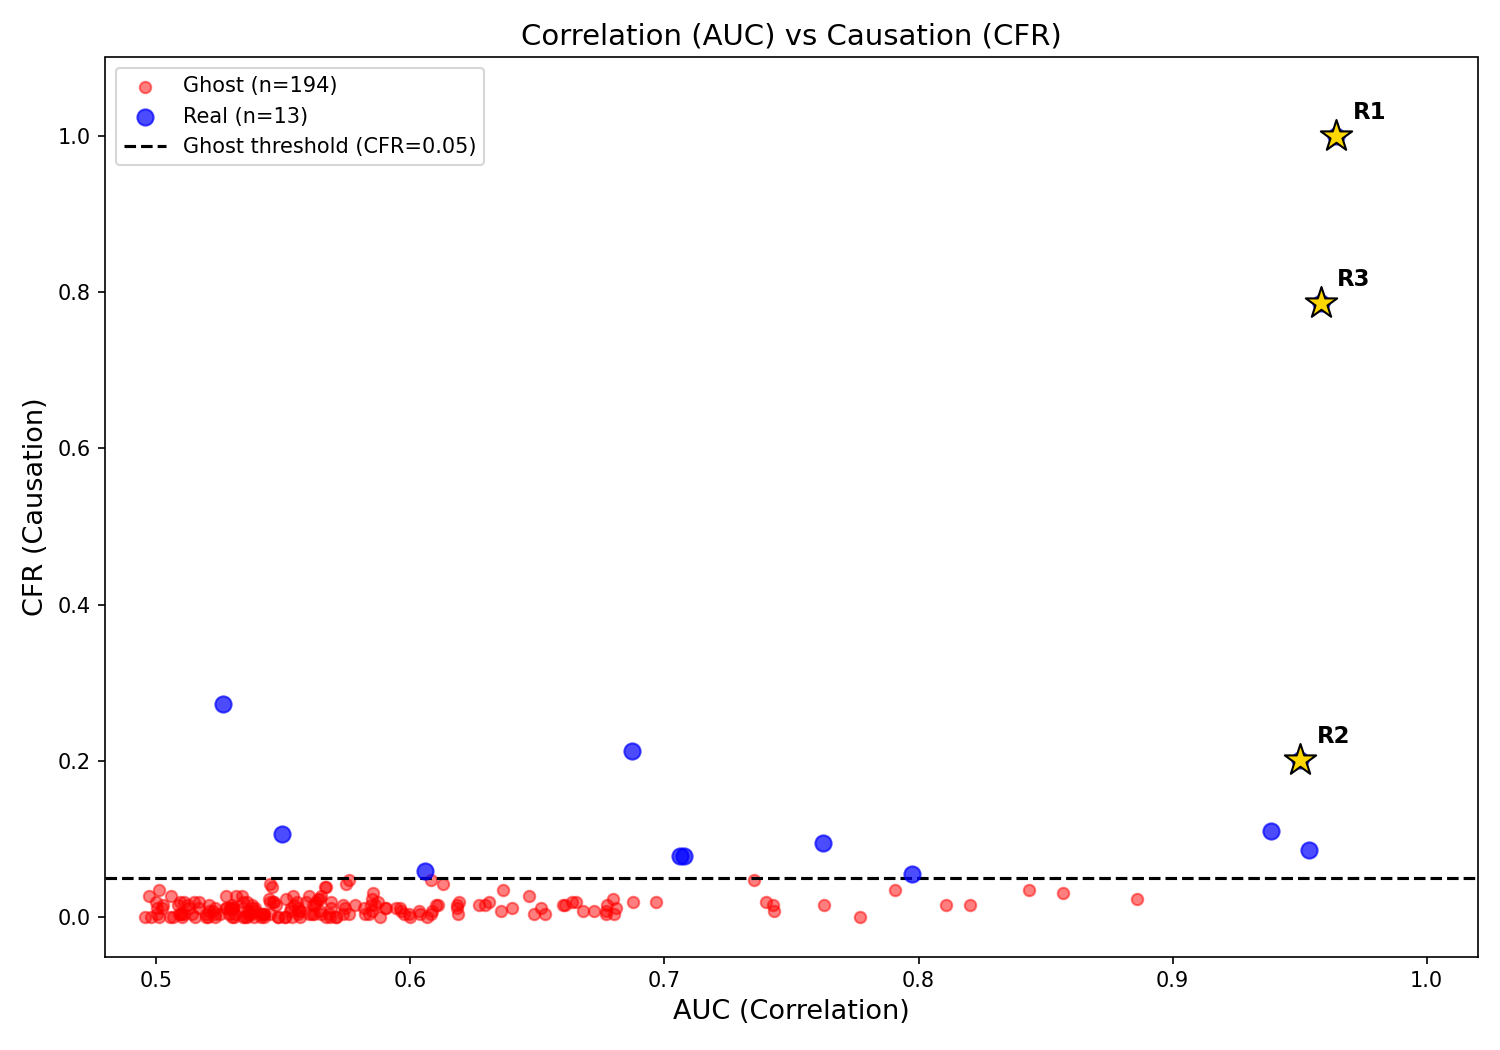
\includegraphics[width=\textwidth]{plot2_auc_vs_cfr.png}
\caption{AUC vs.\ CFR. Many high-AUC directions have zero CFR.}
\end{subfigure}
\caption{CFR ghost detection results.}
\label{fig:cfr_main}
\end{figure}

\begin{figure}[H]
\centering
\begin{subfigure}[b]{0.48\textwidth}
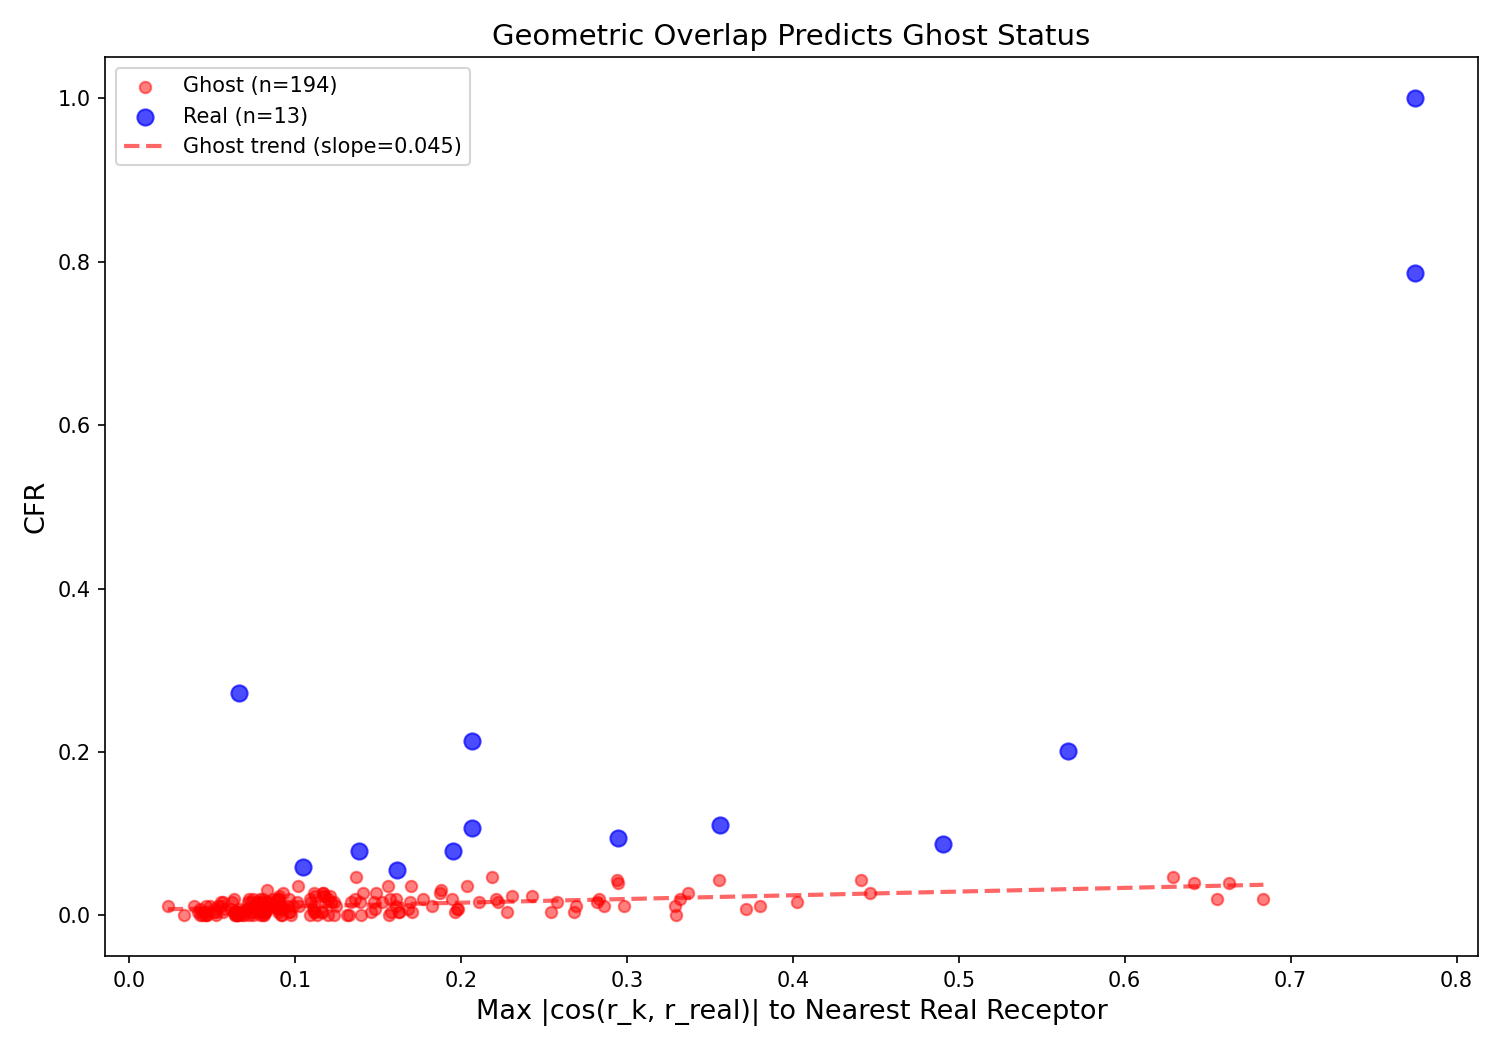
\includegraphics[width=\textwidth]{plot3_cosine_vs_cfr.png}
\caption{Cosine similarity with R1 vs.\ CFR. Ghost directions are often highly aligned with R1.}
\end{subfigure}
\hfill
\begin{subfigure}[b]{0.48\textwidth}
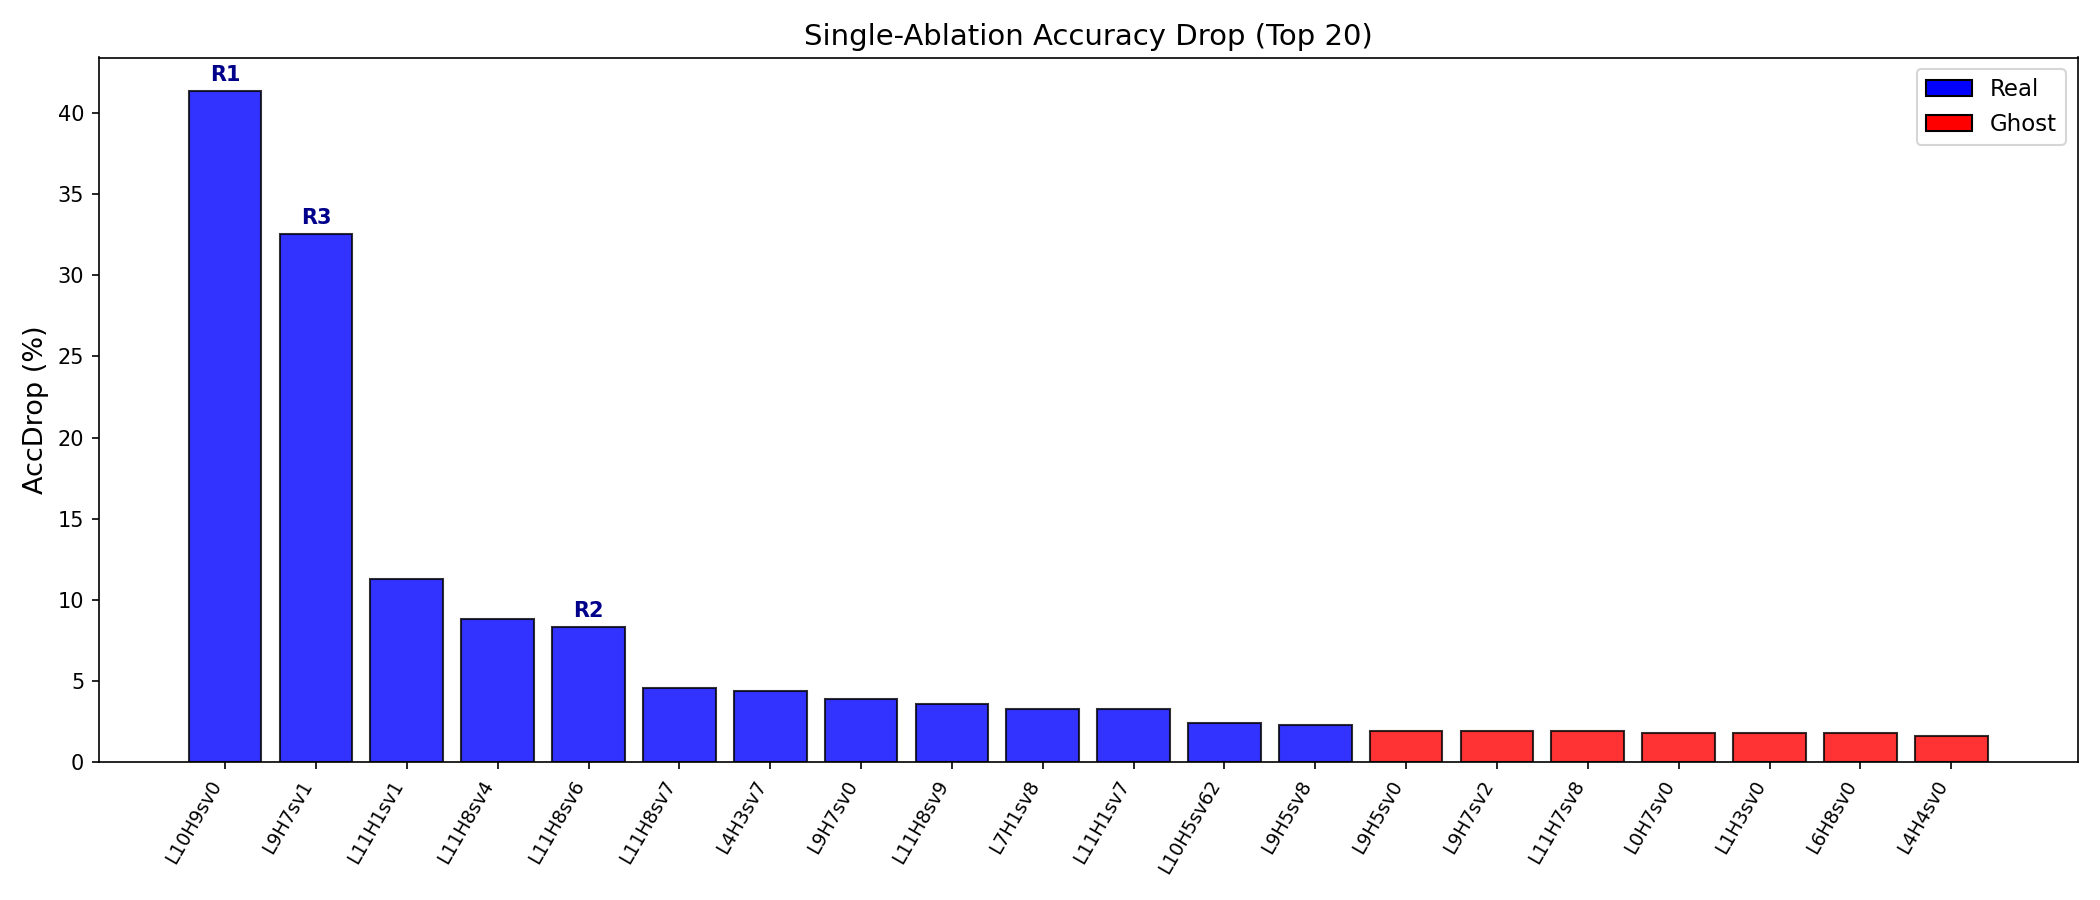
\includegraphics[width=\textwidth]{plot4_accdrop_top20.png}
\caption{Top 20 directions by AccDrop.}
\end{subfigure}
\caption{CFR analysis continued.}
\label{fig:cfr_extra}
\end{figure}

\textbf{194 out of 207 directions are ghosts} (CFR $< 0.1$). The ghost rate is 93.7\%. Only 13 directions survive. This means the mask training vastly over-identifies directions as relevant. The vast majority are \emph{geometric ghosts}---they have high AUC because they are correlated with a real receptor's direction ($\cos > 0.5$ with R1 or R3), not because they carry independent signal.

The cosine plot (Figure~\ref{fig:cfr_extra}a) confirms this: ghost directions cluster at high cosine similarity with R1. They are echoes, not independent signals.

\begin{figure}[H]
\centering
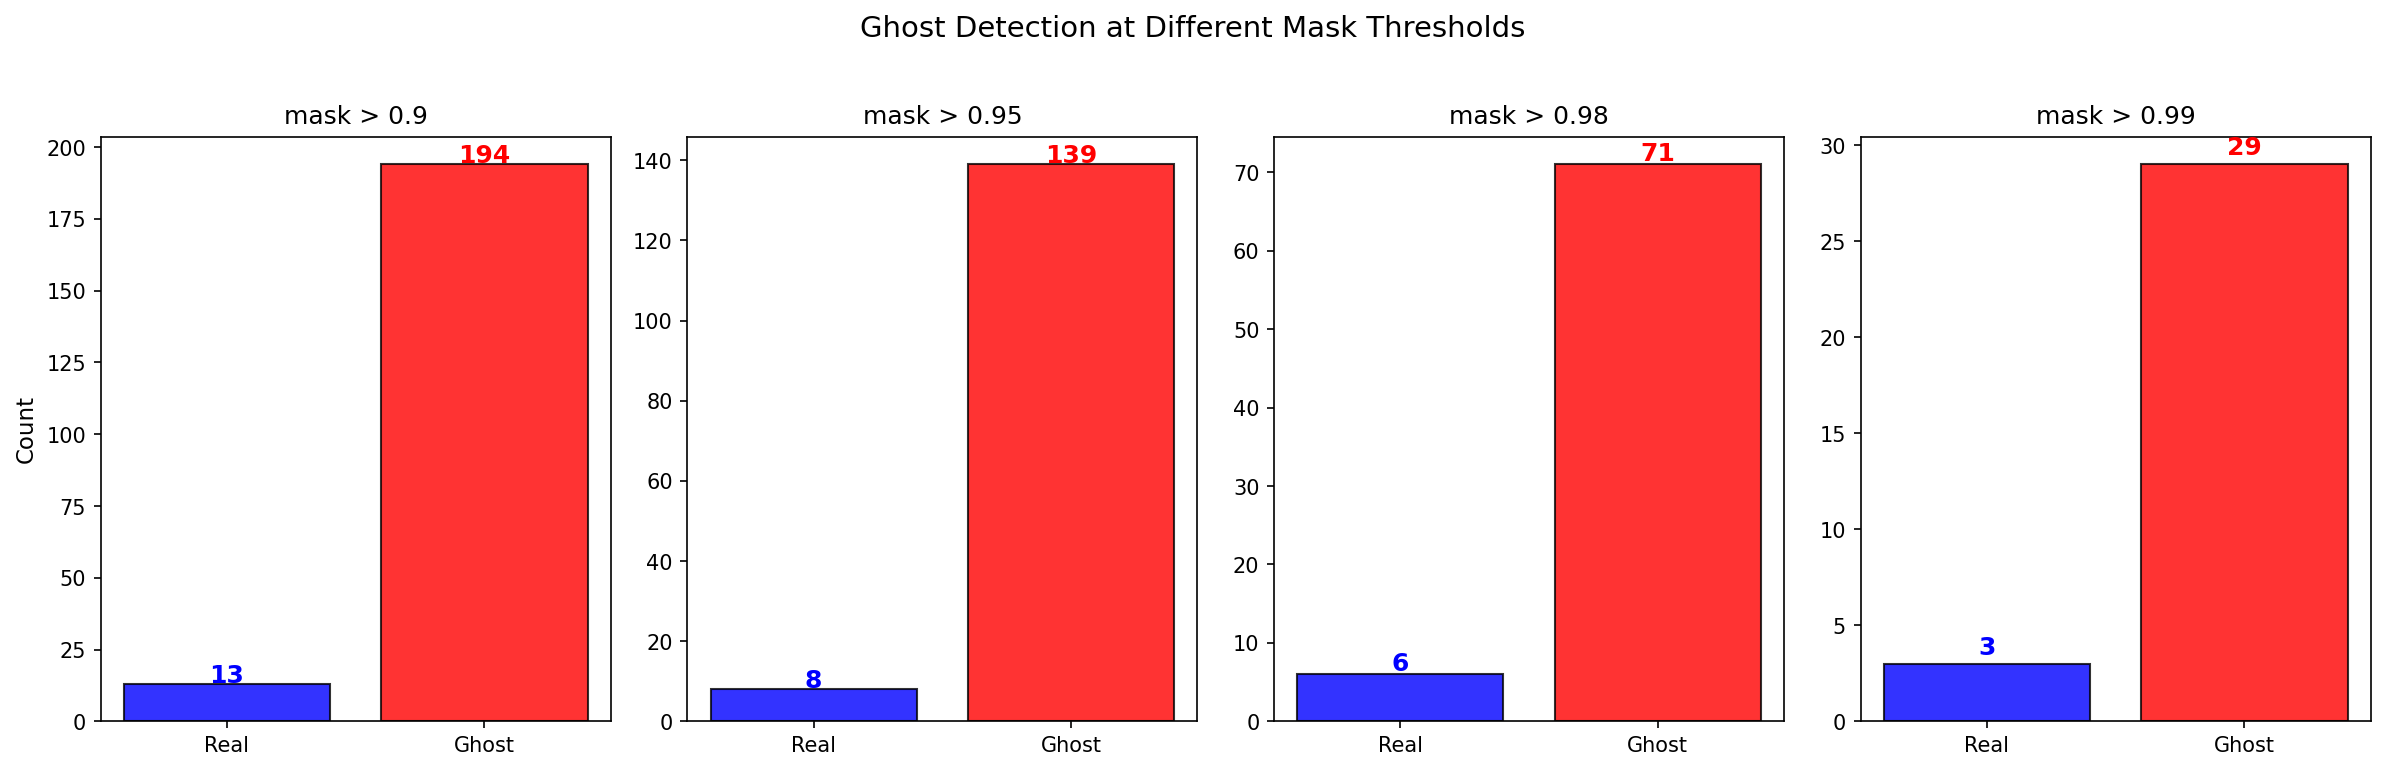
\includegraphics[width=0.6\textwidth]{plot5_thresholds.png}
\caption{Survivor count at different CFR thresholds.}
\label{fig:cfr_threshold}
\end{figure}


%======================================================================
\section{OCA: Orthogonal Component Analysis}
\label{sec:oca}
%======================================================================

CFR reduced 207 to 13 survivors. But are these 13 truly independent, or are some still redundant (correlated with each other)? I developed \emph{Orthogonal Component Analysis} (OCA) to iteratively prune directions that are linearly explained by the current basis.

The algorithm:
\begin{enumerate}[nosep]
\item Sort the 13 CFR survivors by AccDrop (highest first).
\item Initialize the basis $\mathcal{B} = \emptyset$ and the survivor list.
\item For each candidate direction $v$, compute its \emph{independence score}: $\text{Indep}(v) = 1 - \max_{b \in \mathcal{B}} |\cos(v, b)|$. If $\text{Indep}(v) < \tau$ (threshold 0.3), it is a \emph{correlation ghost} and is pruned.
\item Otherwise, add $v$ to $\mathcal{B}$.
\item After processing all candidates, measure total $R^2$: regress the model's logit difference on the activations of the surviving directions.
\end{enumerate}

\subsection{Results}

\begin{figure}[H]
\centering
\begin{subfigure}[b]{0.48\textwidth}
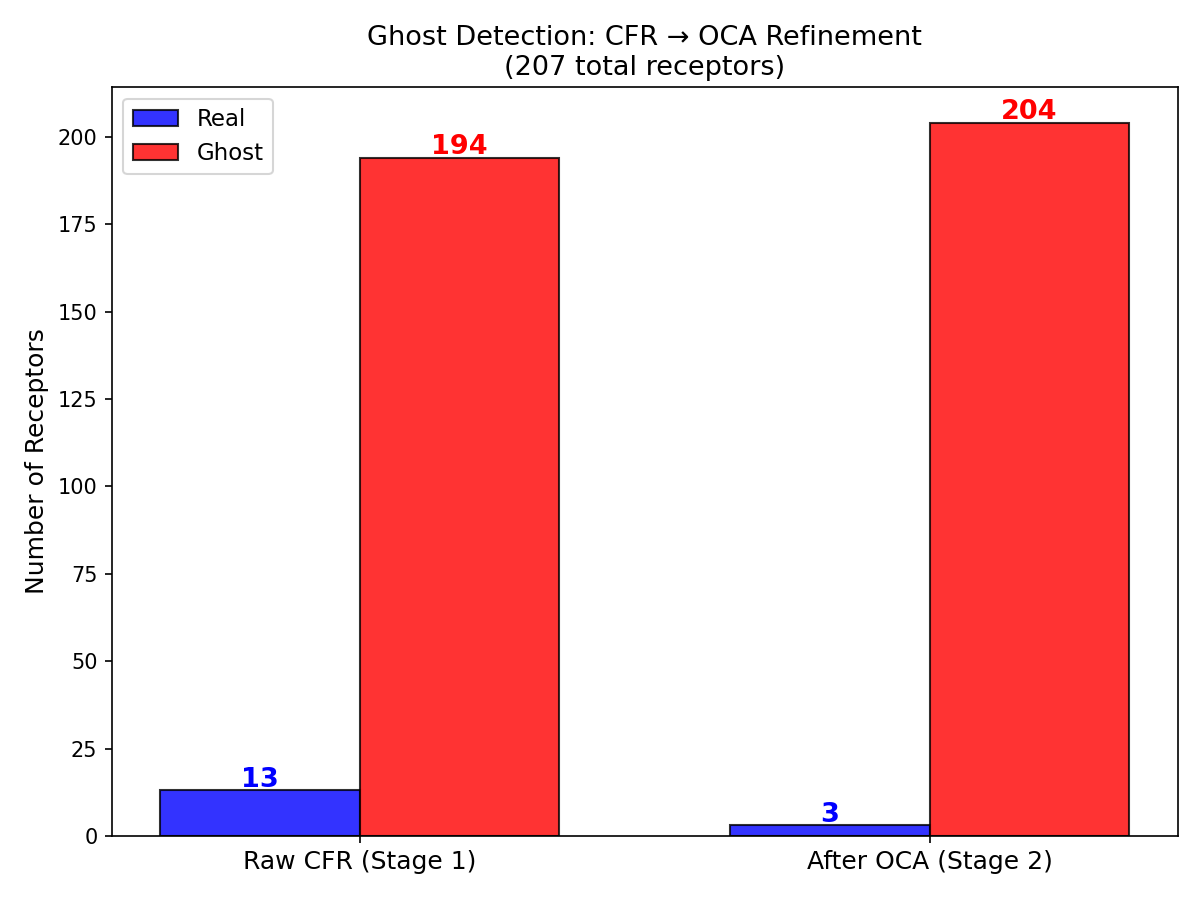
\includegraphics[width=\textwidth]{oca_plot1_before_after.png}
\caption{Before OCA: 13 directions with substantial redundancy. After: 3 independent directions.}
\end{subfigure}
\hfill
\begin{subfigure}[b]{0.48\textwidth}
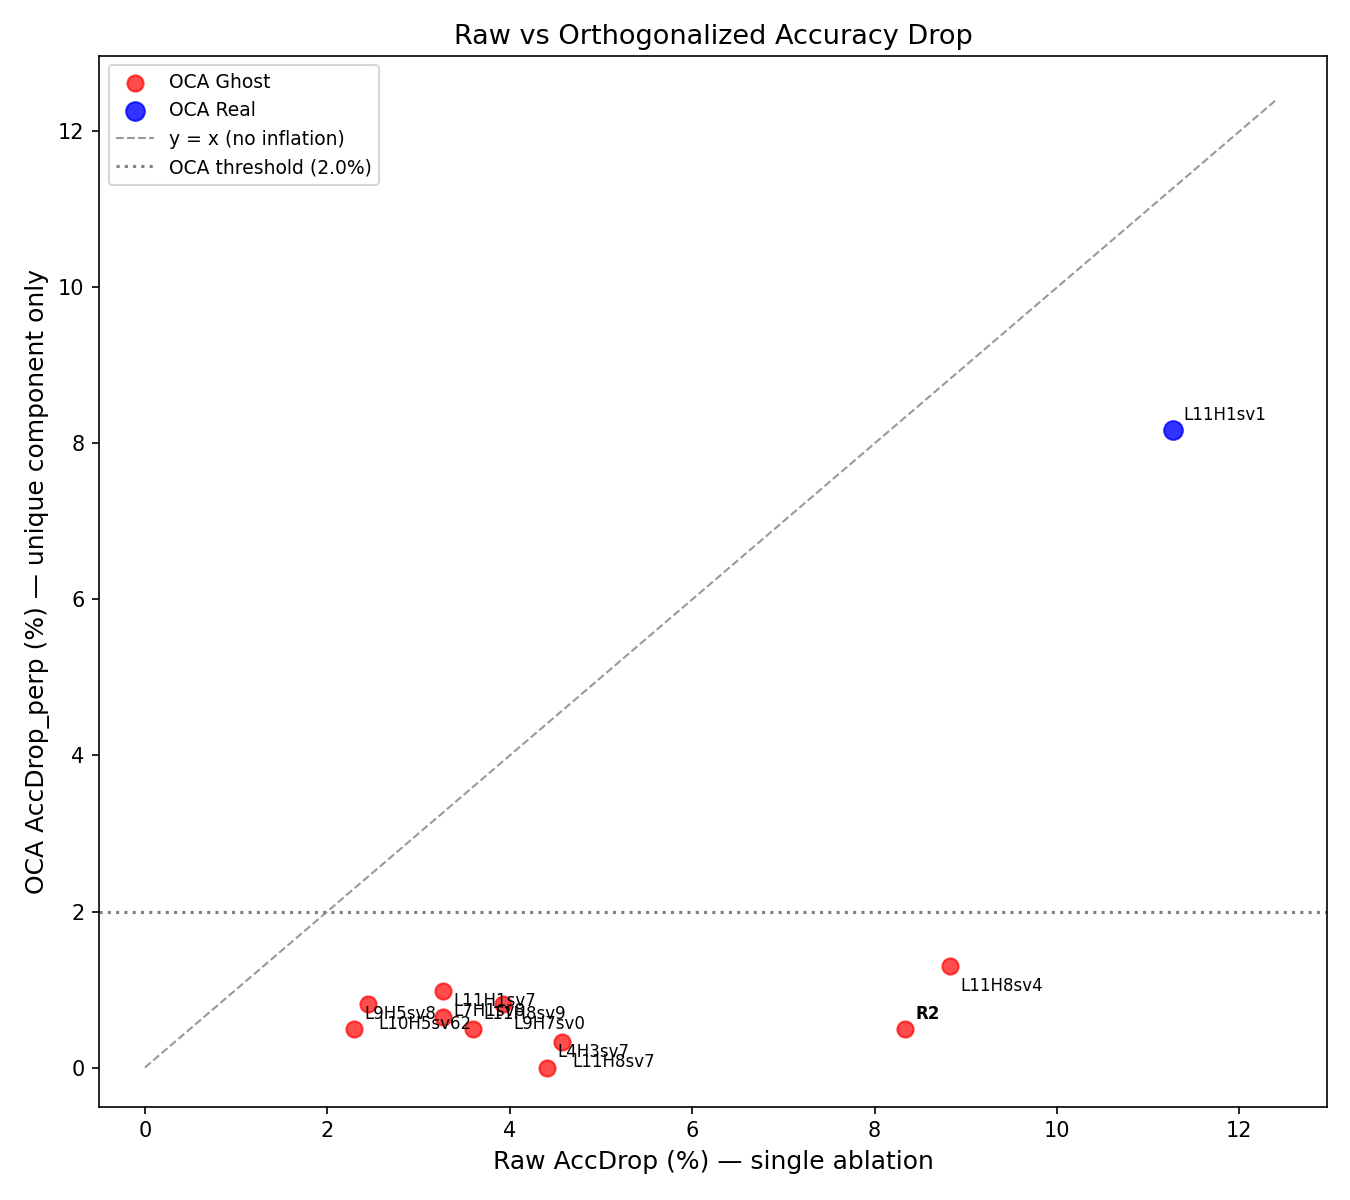
\includegraphics[width=\textwidth]{oca_plot2_raw_vs_oca.png}
\caption{Raw AccDrop vs.\ OCA-filtered AccDrop.}
\end{subfigure}
\caption{OCA refinement: 13 $\to$ 3.}
\label{fig:oca_main}
\end{figure}

\begin{figure}[H]
\centering
\begin{subfigure}[b]{0.48\textwidth}
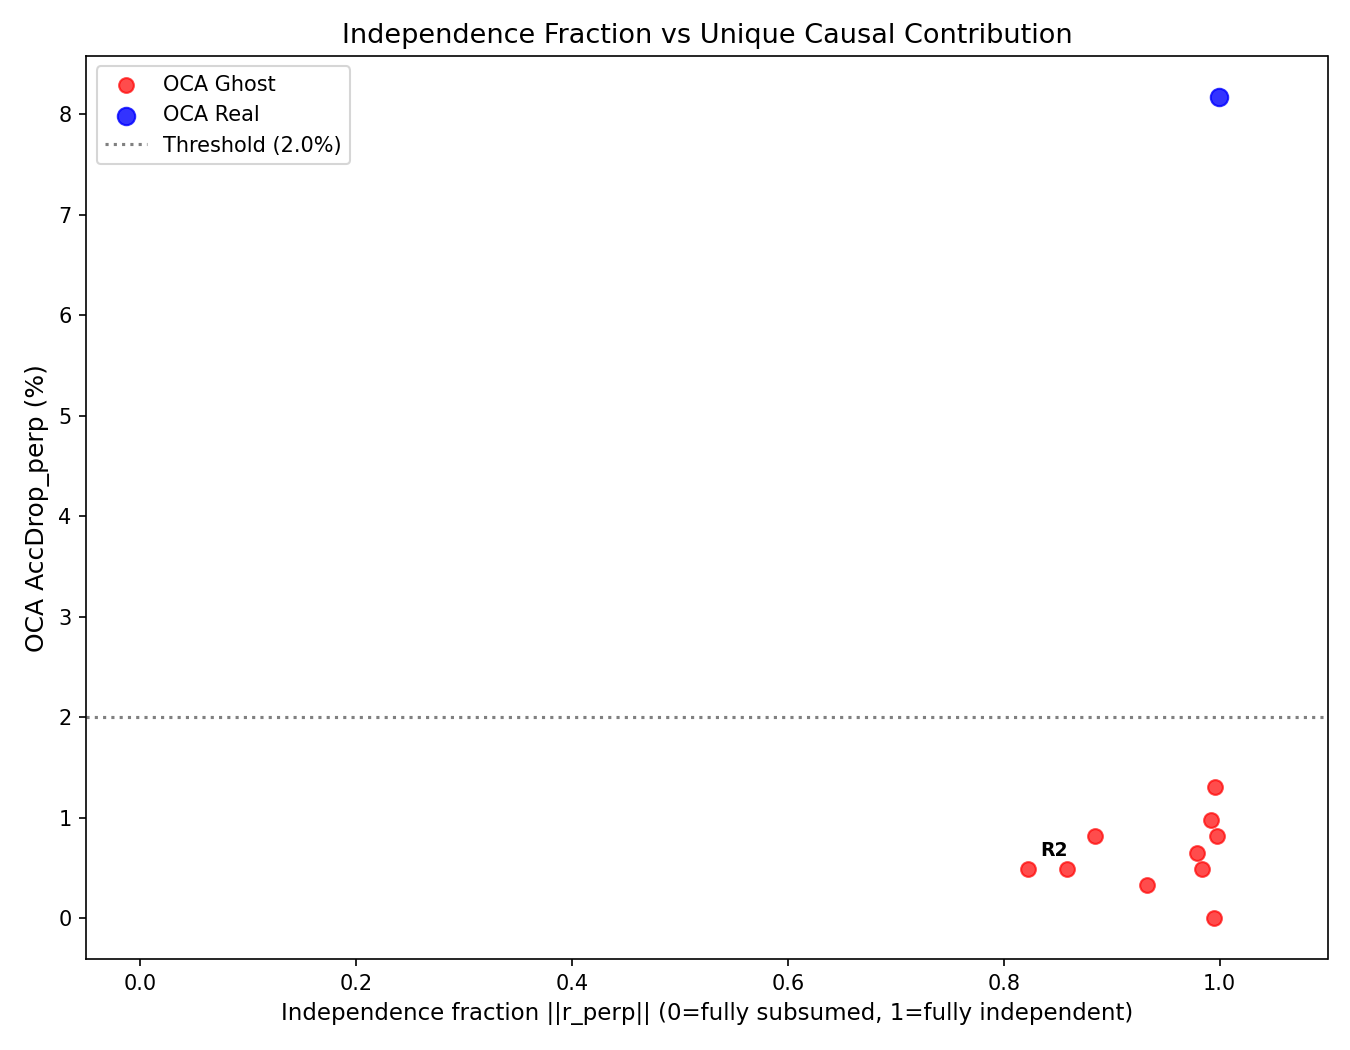
\includegraphics[width=\textwidth]{oca_plot3_independence_vs_accdrop.png}
\caption{Independence score vs.\ AccDrop. Pruned directions (red) have low independence.}
\end{subfigure}
\hfill
\begin{subfigure}[b]{0.48\textwidth}
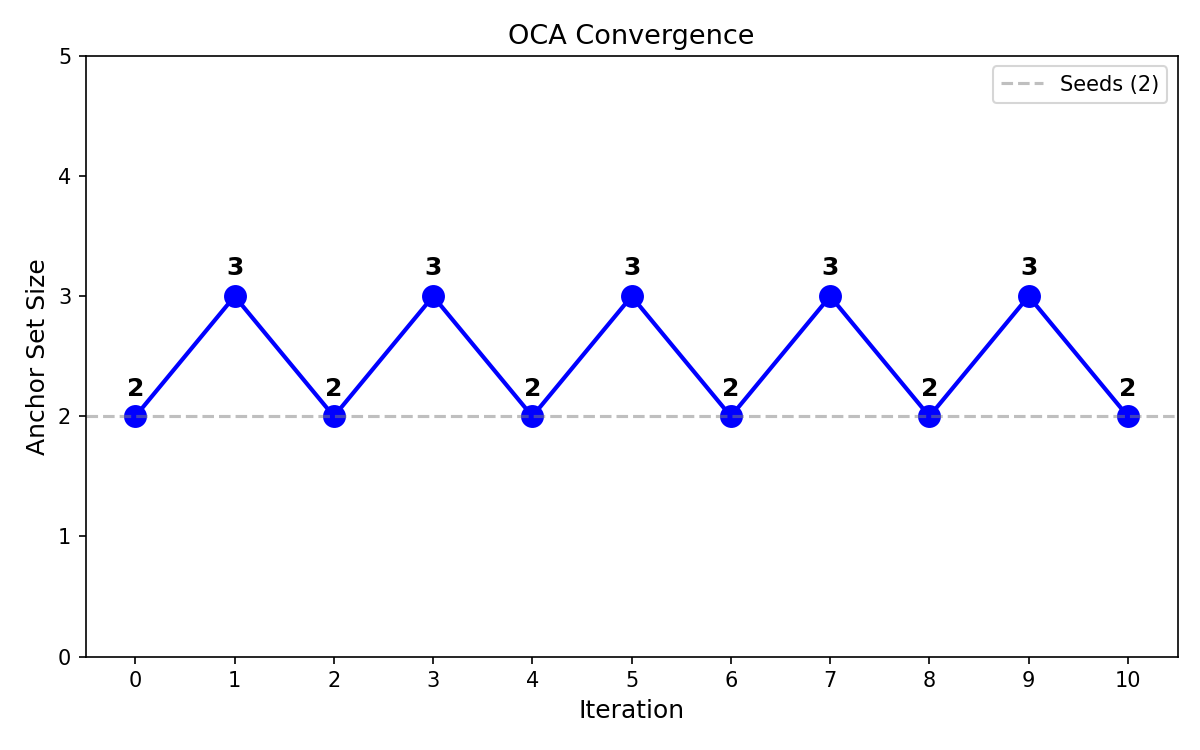
\includegraphics[width=\textwidth]{oca_plot4_convergence.png}
\caption{$R^2$ convergence. Three directions achieve $R^2 = 0.9815$.}
\end{subfigure}
\caption{OCA independence analysis and convergence.}
\label{fig:oca_extra}
\end{figure}

OCA prunes the 13 CFR survivors to exactly 3 independent directions:
\begin{itemize}[nosep]
\item R1: L10H9sv0 (promotion, AccDrop = 3.59\%)
\item R3: L9H7sv1 (inhibition, AccDrop = 1.31\%)
\item \textbf{Dark receptor}: L11H1sv1 (AccDrop = 8.17\%, AUC = 0.526)
\end{itemize}

The combined $R^2 = 0.9815$. Three directions explain 98.15\% of the variance in the model's gender logit difference. The full pipeline---mask training (207) $\to$ CFR (13) $\to$ OCA (3)---achieves a 69$\times$ compression.

The dark receptor is unexpected. It has the \emph{highest} AccDrop (8.17\%) but the \emph{lowest} AUC (0.526, barely above chance for gender classification). Removing it hurts accuracy substantially, yet it does not discriminate between he-contexts and she-contexts. This makes it genuinely interesting: it contributes to the logit variance without encoding gender at the pronoun level.


%======================================================================
\section{Dark Receptor Characterization and PRM}
\label{sec:dark}
%======================================================================

I characterized the dark receptor (L11H1sv1) along three axes: its logit-space profile, its activation distribution by gender context, and its ability to predict model errors.

\subsection{Token Profile}

\begin{figure}[H]
\centering
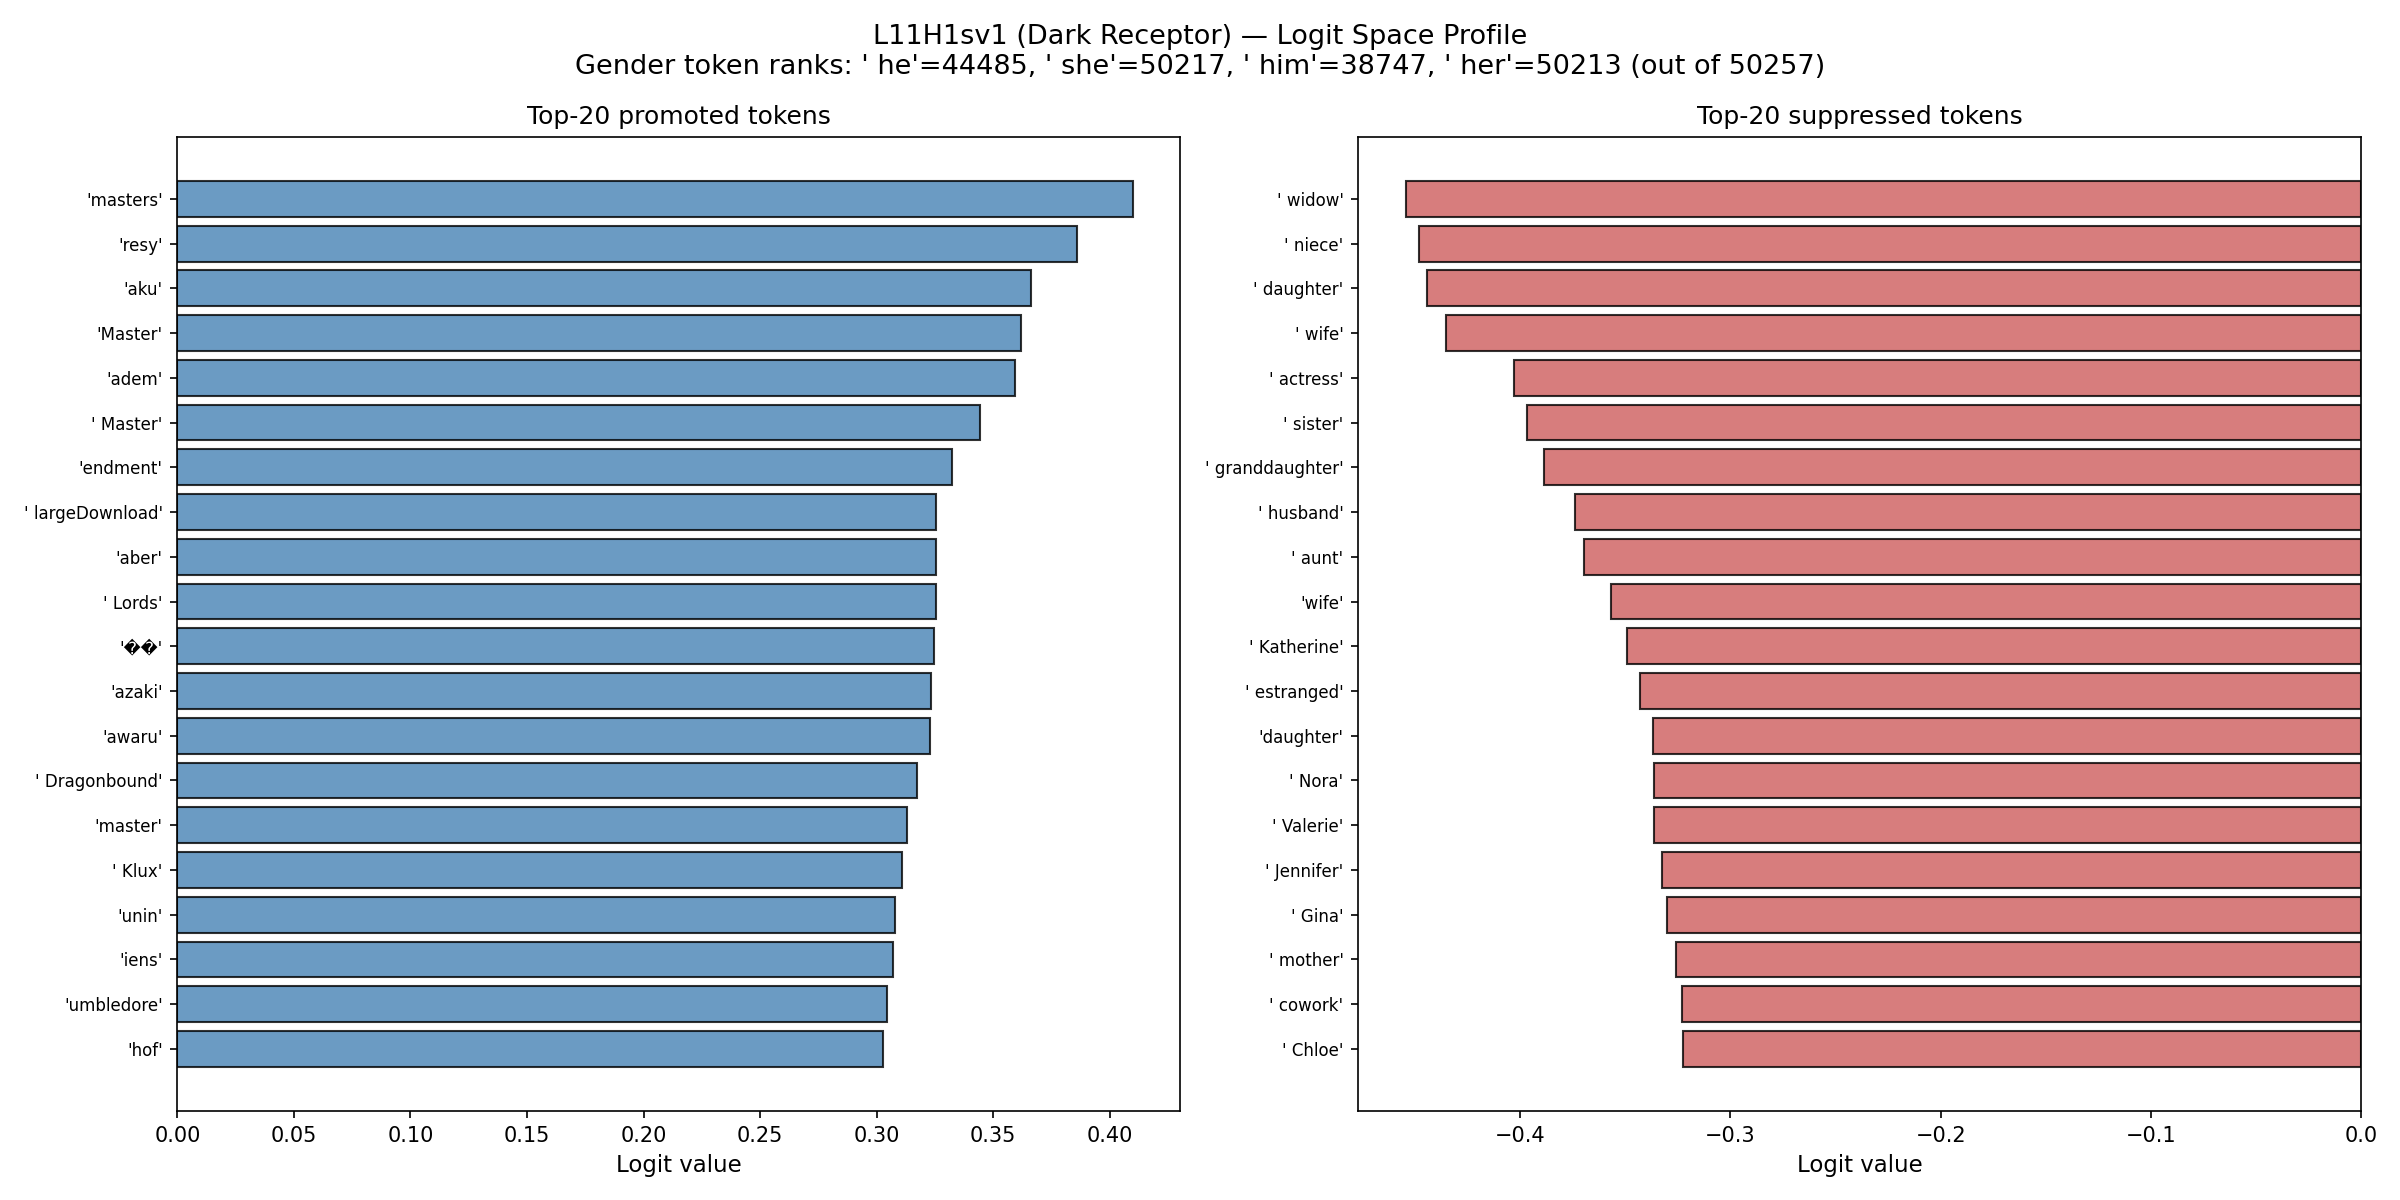
\includegraphics[width=\textwidth]{dark_plot1_token_profile.png}
\caption{Dark receptor logit profile. Top promoted tokens: ``masters'', ``Master'', ``Lords''. Top suppressed tokens: ``widow'', ``niece'', ``daughter'', ``wife''. Pronoun tokens rank near the bottom (``he'' at rank 44485, ``she'' at rank 50217 out of 50257).}
\label{fig:dark_token}
\end{figure}

The dark receptor encodes a \emph{relational-role axis}. It suppresses kinship and relational terms (widow, niece, daughter, wife, sister, granddaughter) and promotes authority/title terms (masters, Master, Lords). Crucially, the actual pronouns (he, she, him, her) are ranked near the very bottom of the 50257-token vocabulary. This direction is orthogonal to the pronoun-gender axis in logit space.

\subsection{Activation Distributions}

\begin{figure}[H]
\centering
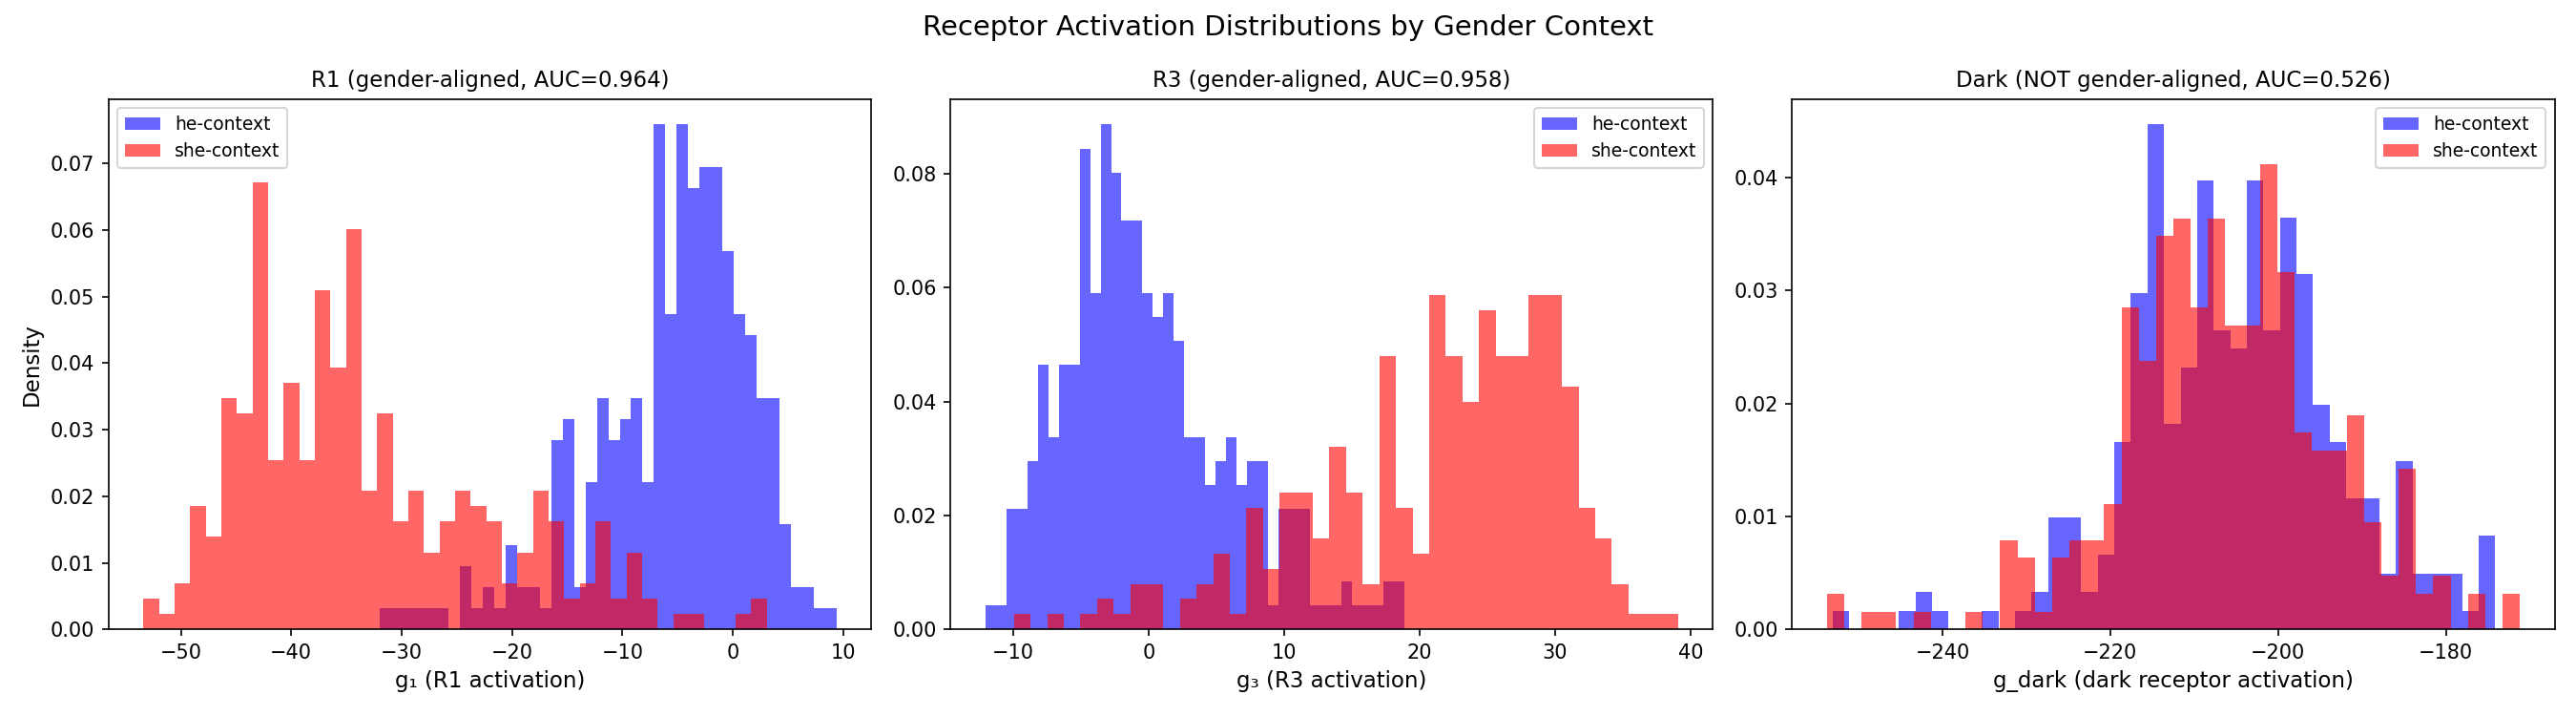
\includegraphics[width=\textwidth]{dark_plot6_distributions.png}
\caption{Receptor activation distributions by gender context. R1 (AUC = 0.964) and R3 (AUC = 0.958) show clean separation. The dark receptor (AUC = 0.526) shows complete overlap.}
\label{fig:dark_dist}
\end{figure}

The dark receptor's activations are nearly constant: mean $= -205.7$, std $= 12.7$ (coefficient of variation 6.2\%). The he-context mean ($-205.1$) and she-context mean ($-206.4$) differ by only $d' = 0.10$. The direction matters for the logit computation (removing it drops accuracy by 8.17\%), but its activation barely varies across examples. This suggests it serves as structural infrastructure---a large constant offset that maintains the global geometry of the residual stream---rather than a per-example discriminative feature.

\subsection{Predictive Receptor Margin: A Null Result}

I hypothesized that the dark receptor might function as a routing or gating signal. If the model needs both gender information (R1, R3) \emph{and} a routing signal (dark receptor) to predict correctly, then errors should cluster where the gender margin is present but the dark signal is weak. I defined three predictors:

\begin{align}
\text{PRM}_2 &= |g_1 - g_3| \quad \text{(gender margin only)} \\
\text{PRM}_3 &= |g_1 - g_3| \times |g_\text{dark}| \quad \text{(gender} \times \text{dark)} \\
\text{PRM}_\text{dark} &= |g_\text{dark}| \quad \text{(dark only)}
\end{align}

I measured their AUC-ROC for predicting model errors (53 errors out of 612 examples, 8.7\% base rate).

\begin{table}[H]
\centering
\begin{tabular}{lcc}
\toprule
Predictor & AUC-ROC & Precision@53 \\
\midrule
PRM$_2$ (gender only) & 0.541 & 1.9\% \\
PRM$_3$ (gender $\times$ dark) & 0.539 & 1.9\% \\
PRM$_\text{dark}$ (dark only) & 0.544 & 3.8\% \\
\midrule
Random baseline & 0.500 & 8.7\% \\
\bottomrule
\end{tabular}
\caption{Error prediction performance. All predictors perform at chance. PRM$_3$ is worse than PRM$_2$---adding the dark receptor \emph{hurts}.}
\label{tab:prm}
\end{table}

\begin{figure}[H]
\centering
\begin{subfigure}[b]{0.48\textwidth}
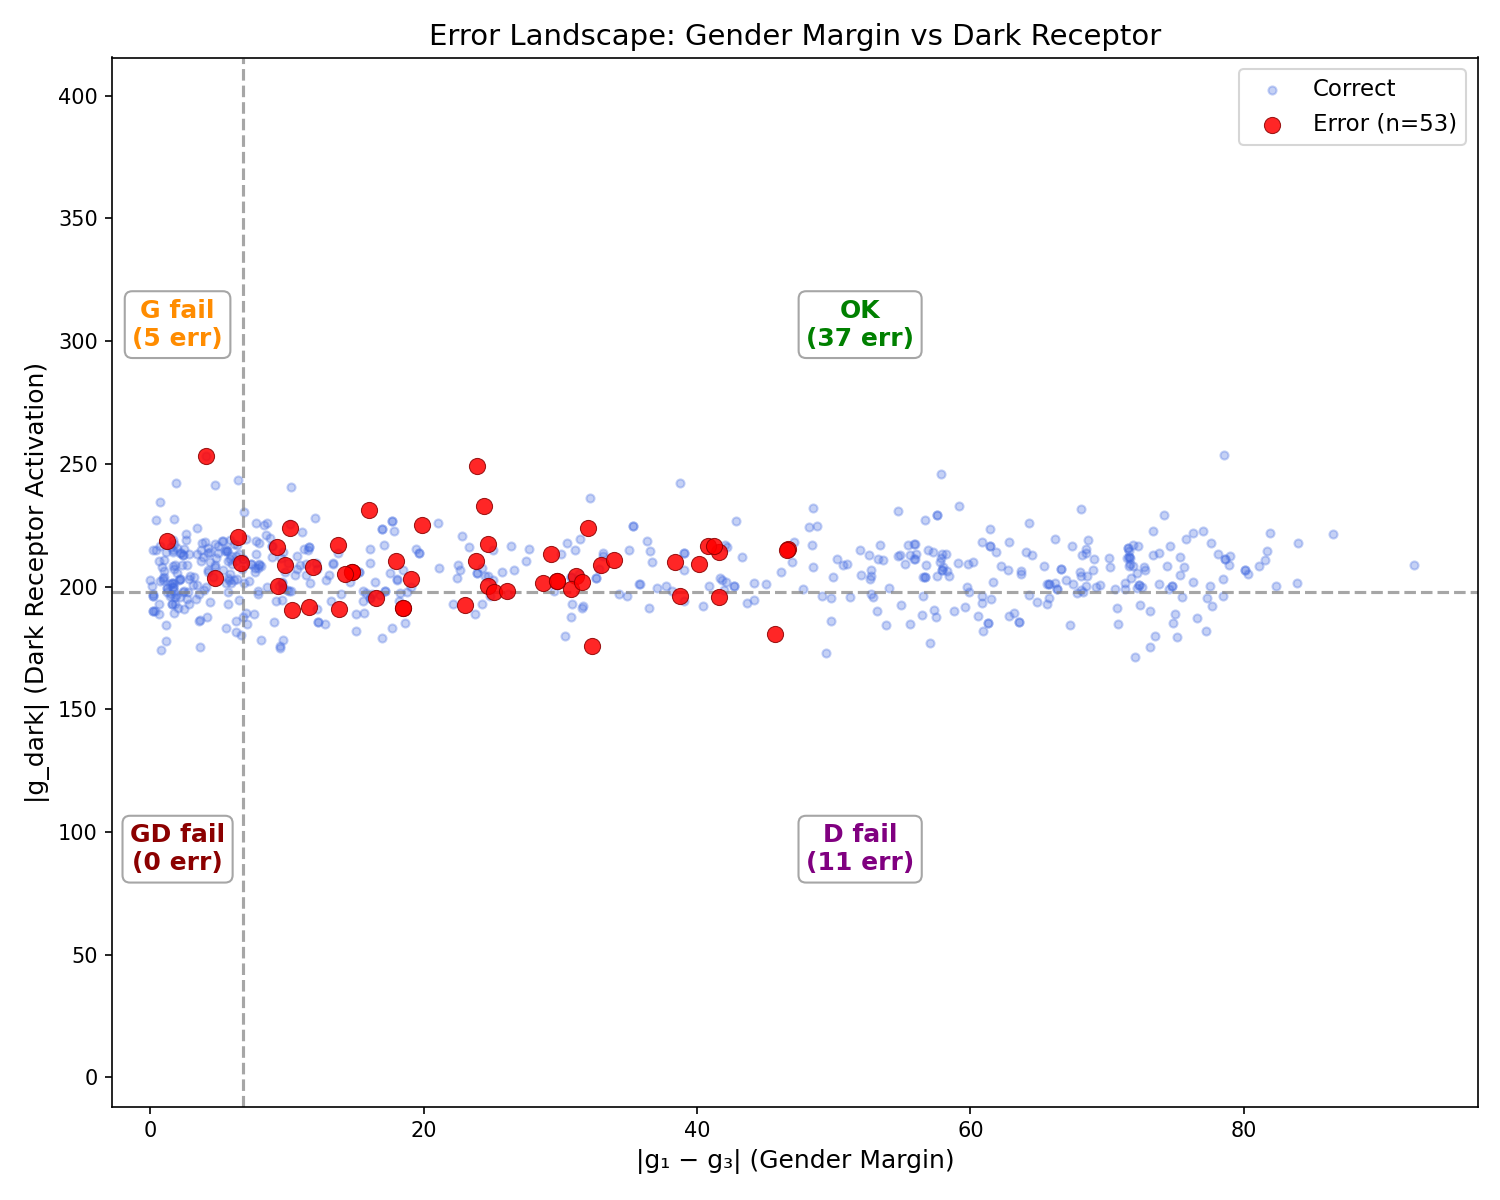
\includegraphics[width=\textwidth]{dark_plot2_error_landscape.png}
\caption{Error landscape. Errors are scattered uniformly; no clustering in any quadrant.}
\end{subfigure}
\hfill
\begin{subfigure}[b]{0.48\textwidth}
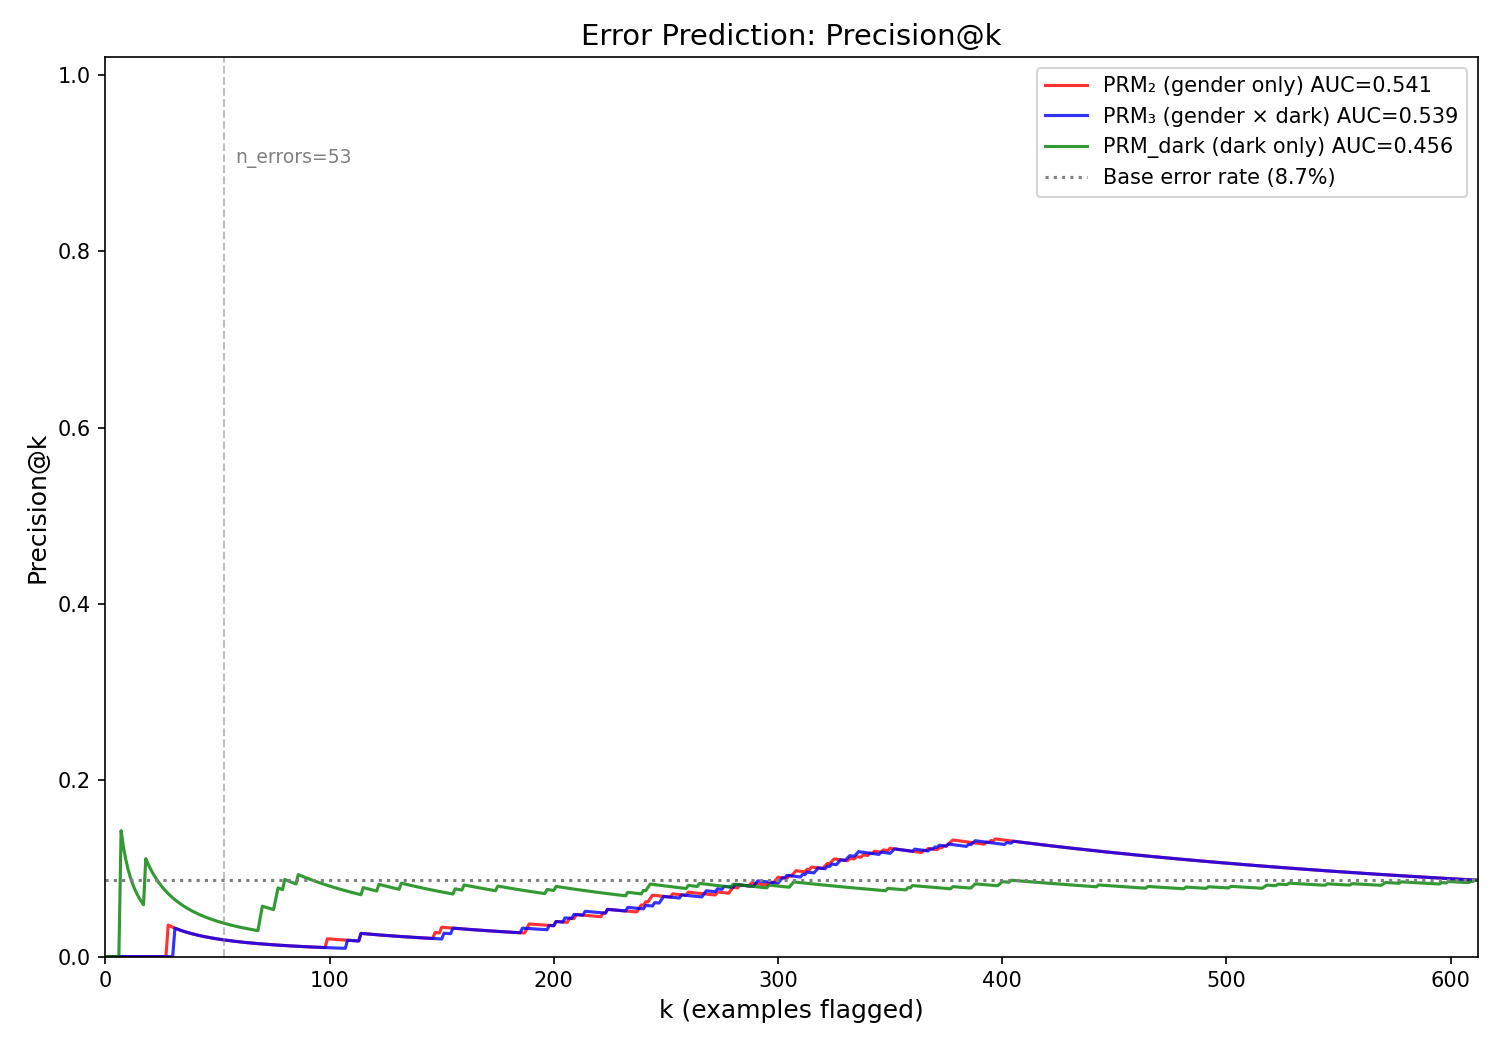
\includegraphics[width=\textwidth]{dark_plot3_precision_at_k.png}
\caption{Precision@$k$. All three predictors hover near or below the base rate.}
\end{subfigure}
\caption{PRM error prediction: a null result.}
\label{fig:prm_fail}
\end{figure}

The hypothesis failed. AUCs of 0.54 are functionally chance. PRM$_3$ performs \emph{worse} than PRM$_2$ by 0.002. The dark receptor adds zero predictive value for identifying which examples the model gets wrong.

I also decomposed errors by failure type (gender margin below threshold, dark activation below threshold, both, or neither). The results contradicted the hypothesis: the ``OK'' quadrant (both signals strong) had the \emph{highest} error rate (10.7\%), while ``both fail'' had zero errors. The thresholds may be wrong, or the hypothesis is fundamentally flawed.

\paragraph{Interpretation.} The dark receptor contributes to logit variance (hence AccDrop = 8.17\% and $R^2 = 0.98$) but not in a way that predicts individual failures. Its large mean activation ($-205$) and small variance (std = 12.7) suggest it acts as a global calibration term. Removing it shifts the entire logit distribution, disrupting ln\_final's normalization for all examples simultaneously. This is a \emph{global} effect, not a per-example gating mechanism.

I consider this experiment a clean null result. The dark receptor exists, it matters causally, and its token profile is interpretable (relational-role axis). But it does not function as a routing signal, and the PRM framework does not predict errors on this task.


%======================================================================
\section{Summary of Findings}
\label{sec:summary}
%======================================================================

Across twelve experiments, the following picture emerges.

The GP circuit in GPT-2 Small operates through three independent directions in the residual stream. R1 (L10H9sv0) inherits gender information from the token embedding and serves as the primary promotion channel. R3 (L9H7sv1) computes an inhibition signal at layer 9, providing the sharpest gender discrimination. A third ``dark'' direction (L11H1sv1) contributes to the global logit geometry without encoding pronoun gender.

These three directions explain 98.15\% of the variance in the model's he-vs-she logit difference. Out of 207 mask-identified directions, 93.7\% are ghosts---directions that appear gender-aligned only because they are geometrically correlated with a real receptor. The CFR + OCA pipeline compresses the representation from 207 to 3 without meaningful information loss.

The circuit's errors are dominated by margin failures (52\% of errors), where both receptors vote correctly but with insufficient confidence. Ambiguous names (he-fraction near 0.5) drive most of these failures. The receptor directions generalize across five syntactic structures with AUC $\geq 0.92$ in all cases.

Cross-talk between R1 and R3 is 41\% computational (beyond geometric projection), confirming that the circuit is not a set of independent channels but a coupled system with directional information flow from R3 (layer 9) to R1 (layer 10).


%======================================================================
\section{Next Steps}
\label{sec:next}
%======================================================================

Several directions remain open. First, testing whether the GP receptor directions transfer to the Indirect Object Identification (IOI) task would address whether these directions are task-specific or reflect general gender representations in the model. I expect R1 to transfer (since it inherits from the embedding) and R3 not to (since it is computed by a specific head for a specific task).

Second, formalizing the cross-talk matrix from Experiment 2 as a \emph{Receptor Interaction Matrix} (RIM) would provide a compact, reusable object that characterizes how receptors couple through intermediate computation.

Third, scaling the CFR + OCA pipeline to a larger model (GPT-2 Medium or GPT-2 Large) would test whether the ghost phenomenon persists and whether the compression ratio holds.

\end{document}
